% arara: pdflatex: { shell: on }
% arara: biber
% arara: pdflatex: { shell: on }
% arara: pdflatex: { shell: on }
%% arara: biber
%% arara: pdflatex: { shell: on }
%% arara: pdflatex: { shell: on }
% arara: clean: { files: [ Masterarbeit_Grieco_1408410.aux, Masterarbeit_Grieco_1408410.bbl, Masterarbeit_Grieco_1408410.bcf, Masterarbeit_Grieco_1408410.cod, Masterarbeit_Grieco_1408410.blg, Masterarbeit_Grieco_1408410.lof, Masterarbeit_Grieco_1408410.lot, Masterarbeit_Grieco_1408410.out, Masterarbeit_Grieco_1408410.toc, Masterarbeit_Grieco_1408410.log, Masterarbeit_Grieco_1408410.lol, Masterarbeit_Grieco_1408410.run.xml, Masterarbeit_Grieco_1408410.listing] } 

% ------------------------------------------------------------------------------
% Formatvorlage f?r Masterarbeiten an der Ohm-Hochschule N?rnberg
% ------------------------------------------------------------------------------
%   erstellt von Stefan Macke, 24.04.2009
%   http://blog.stefan-macke.de
% Dokumentenkopf ---------------------------------------------------------------
%   Diese Vorlage basiert auf "scrreprt" aus dem koma-script.
% ------------------------------------------------------------------------------

\documentclass[
    12pt, % Schriftgröße
    DIV10,
    ngerman, % für Umlaute, Silbentrennung etc.
    a4paper, % Papierformat
    oneside, % einseitiges Dokument
    titlepage, % es wird eine Titelseite verwendet
    parskip=half, % Abstand zwischen Absätzen (halbe Zeile)
    headings=normal, % Größe der Überschriften verkleinern
    listof=totoc, % Verzeichnisse im Inhaltsverzeichnis aufführen
    listof=entryprefix,
    bibliography=totoc, % Literaturverzeichnis im Inhaltsverzeichnis aufführen
    index=totoc, % Index im Inhaltsverzeichnis aufführen
    captions=tableheading, % Beschriftung von Tabellen unterhalb ausgeben
    final % Status des Dokuments (final/draft)
]{scrreprt}

% Weise compiler an, nicht bei Fehlern anzuhalten!
% \nonstopmode

% Meta-Informationen -----------------------------------------------------------
%   Informationen über das Dokument, wie z.B. Titel, Autor, Matrikelnr. etc
%   werden in der Datei Meta.tex definiert und können danach global
%   verwendet werden.
% ------------------------------------------------------------------------------
% Meta-Informationen -----------------------------------------------------------
%   Definition von globalen Parametern, die im gesamten Dokument verwendet
%   werden k�nnen (z.B auf dem Deckblatt etc.).
%
%   ACHTUNG: Wenn die Texte Umlaute oder ein Esszet enthalten, muss der folgende
%            Befehl bereits an dieser Stelle aktiviert werden:
%            \usepackage[latin1]{inputenc}
% ------------------------------------------------------------------------------

\newcommand{\mytitel}{Programmiersprachliche Konzepte von COBOL im Vergleich mit Java -- Eine praxisorientierte Einf�hrung}
\newcommand{\myart}{Masterarbeit}
\newcommand{\myfachgebiet}{Informatik und Multimedia}
\newcommand{\myautor}{Antonio Grieco}
\newcommand{\mymatrikelnr}{}
\newcommand{\myerstgutachter}{}
\newcommand{\myzweitgutachter}{}
\newcommand{\myjahr}{2018}
\newcommand{\myort}{Augsburg}

% benötigte Packages -----------------------------------------------------------
%   LaTeX-Packages, die benötigt werden, sind in die Datei Packages.tex
%   "ausgelagert", um diese Vorlage möglichst übersichtlich zu halten.
% ------------------------------------------------------------------------------
% Anpassung des Seitenlayouts --------------------------------------------------
%   siehe Seitenstil.tex
% ------------------------------------------------------------------------------
\usepackage[
    automark, % Kapitelangaben in Kopfzeile automatisch erstellen
    headsepline, % Trennlinie unter Kopfzeile
    ilines % Trennlinie linksbündig ausrichten
]{scrlayer-scrpage}

% Anpassung an Landessprache ---------------------------------------------------
\usepackage[ngerman,showlanguages]{babel}

% Umlaute ----------------------------------------------------------------------
%   Umlaute/Sonderzeichen wie äüöß direkt im Quelltext verwenden (CodePage).
%   Erlaubt automatische Trennung von Worten mit Umlauten.
% ------------------------------------------------------------------------------
\usepackage[utf8]{inputenc}
\usepackage[T1]{fontenc}
\usepackage{textcomp} % Euro-Zeichen etc.

% Schrift ----------------------------------------------------------------------
\usepackage{lmodern} % bessere Fonts
\usepackage{relsize} % Schriftgröße relativ festlegen

% Grafiken ---------------------------------------------------------------------
% Einbinden von JPG-Grafiken ermöglichen
%\usepackage[dvips,final]{graphicx}
% hier liegen die Bilder des Dokuments
%\graphicspath{{Bilder/}}

% Befehle aus AMSTeX für mathematische Symbole z.B. \boldsymbol \mathbb --------
\usepackage{amsmath,amsfonts}

% für Index-Ausgabe mit \printindex --------------------------------------------
\usepackage{makeidx}
\makeindex
\AtBeginDocument{\renewcommand\indexname{Stichwortverzeichnis}}
%\addcontentsline{toc}{chapter}{Stichwortverzeichnis}

% Einfache Definition der Zeilenabstände und Seitenränder etc. -----------------
\usepackage{setspace}
\usepackage{geometry}

% Symbolverzeichnis ------------------------------------------------------------
%   Symbolverzeichnisse bequem erstellen. Beruht auf MakeIndex:
%     makeindex.exe %Name%.nlo -s nomencl.ist -o %Name%.nls
%   erzeugt dann das Verzeichnis. Dieser Befehl kann z.B. im TeXnicCenter
%   als Postprozessor eingetragen werden, damit er nicht ständig manuell
%   ausgeführt werden muss.
%   Die Definitionen sind ausgegliedert in die Datei "Glossar.tex".
% ------------------------------------------------------------------------------
% \usepackage[intoc]{nomencl}
% \let\abbrev\nomenclature
% \renewcommand{\nomname}{Abkürzungsverzeichnis}
% \setlength{\nomlabelwidth}{.25\hsize}
% \renewcommand{\nomlabel}[1]{#1 \dotfill}
% \setlength{\nomitemsep}{-\parsep}

% Abkürzungsverzeichnis
\usepackage[printonlyused]{acronym} %Abkürzungsverzeichnis erstellen, Langtext als Fußnote, Auflistung nur bei Verwendung

% zum Umfließen von Bildern ----------------------------------------------------
\usepackage{floatflt}
\usepackage{float}

% Abstand der float caption
\usepackage{caption}
\captionsetup{belowskip=10pt,aboveskip=10pt}

% ensure floats do not go into the next section.
\usepackage[section]{placeins}

% Farben
\usepackage[dvipsnames]{xcolor}
\definecolor{hellgrau}{rgb}{0.93,0.93,0.93}
\definecolor{colKeys}{rgb}{0,0,0.9}
\definecolor{colIdentifier}{rgb}{0,0,0}
\definecolor{colComments}{rgb}{0.6,0,0}
\definecolor{colString}{rgb}{0,0.7,0}

% Farben für Java Diagram
\definecolor{javaProgramm}  {rgb}{0.95, 0.9,    0.5}
\definecolor{javaPackage}   {rgb}{0,    0.7,    0}
\definecolor{javaClass}     {rgb}{0,    0.7,    0.7}
\definecolor{javaAnonClass} {rgb}{0.1,  0.7,    0.7}
\definecolor{javaMethod}    {rgb}{0.7,  0,      0}
\definecolor{javaStatement} {rgb}{1,    0.5,    0}

% zum Einbinden von Programmcode -----------------------------------------------
\usepackage{listings}
\usepackage[newfloat]{minted}

\setminted{
    xleftmargin=20pt,
    linenos=true,
    breaklines
}

\lstset{
    float=hbp,
    basicstyle=\ttfamily\color{black}\small\smaller,
    keywordstyle=\color{colKeys},
    stringstyle=\color{colString},
    commentstyle=\color{colComments},
    columns=flexible,
    tabsize=4,
    frame=single,
    extendedchars=true,
    showspaces=false,
    showstringspaces=false,
    numbers=left,
    numberstyle=\tiny,
    breaklines=true,
    backgroundcolor=\color{hellgrau},
    captionpos=b,
    breakautoindent=true
}

% URL verlinken, lange URLs umbrechen etc. -------------------------------------
\usepackage{url}
\makeatletter
\g@addto@macro{\UrlBreaks}{\UrlOrds}
\makeatother

%% Roman pagenumbers good aligned in toc
%\usepackage{tocloft}
%\cftsetpnumwidth{2em}
%\setlength\cftafterfigskip{10pt}
%\renewcommand\cftchapafterpnum{\vskip10pt}
%\renewcommand\cftsecafterpnum{\vskip15pt}

% fortlaufendes Durchnummerieren der Fußnoten ----------------------------------
\usepackage{chngcntr}

% für lange Tabellen -----------------------------------------------------------
\usepackage{longtable}
\usepackage{array}
\usepackage{ragged2e}

% seiten rotieren
\usepackage{pdflscape}

% Spaltendefinition rechtsbündig mit definierter Breite ------------------------
\newcolumntype{w}[1]{>{\raggedleft\hspace{0pt}}p{#1}}

% Formatierung von Listen ändern -----------------------------------------------
\usepackage{paralist}

% bei der Definition eigener Befehle benötigt
\usepackage{ifthen}

% definiert u.a. die Befehle \todo und \listoftodos
\usepackage{todonotes}

% sorgt dafür, dass Leerzeichen hinter parameterlosen Makros nicht als Makroendezeichen interpretiert werden
\usepackage{xspace}

% einbinden anderer PDF Dateien (Deckblatt etc.)
\usepackage{pdfpages}

% Bibliographics
% Naturwissenschaftliche Bibliographien
%\usepackage[square, comma, numbers]{natbib}
% Stil der Zitate und der Bibliographie
%\bibliographystyle{natdin}
\usepackage[backend=biber]{biblatex}
\addbibresource{Sonstiges/Literatur.bib}

% Tikz libraries
\usepackage{tikz}
\usetikzlibrary{patterns}
\usepackage{tikz-uml}

% Spalten
\usepackage{multicol}

% Anhang
\usepackage[toc,page]{appendix}

% SVG Biler
\usepackage{svg}

% euro sign
\usepackage{eurosym}

% subfigures
\usepackage{subfig}
\usepackage{floatflt}
\usepackage{wrapfig}

% Quotes in babel language
\usepackage{csquotes}


% PDF-Optionen -----------------------------------------------------------------
\usepackage[
    bookmarks,
    bookmarksopen=true,
    colorlinks=true,
% diese Farbdefinitionen zeichnen Links im PDF farblich aus
    linkcolor=black, % einfache interne Verknüpfungen
    anchorcolor=black,% Ankertext
    citecolor=black, % Verweise auf Literaturverzeichniseinträge im Text
    filecolor=black, % Verknüpfungen, die lokale Dateien öffnen
    menucolor=black, % Acrobat-Menüpunkte
    urlcolor=black, 
% diese Farbdefinitionen sollten für den Druck verwendet werden (alles schwarz)
    %linkcolor=black, % einfache interne Verknüpfungen
    %anchorcolor=black, % Ankertext
    %citecolor=black, % Verweise auf Literaturverzeichniseinträge im Text
    %filecolor=black, % Verknüpfungen, die lokale Dateien öffnen
    %menucolor=black, % Acrobat-Menüpunkte
    %urlcolor=black,
    plainpages=false, % zur korrekten Erstellung der Bookmarks
    pdfpagelabels, % zur korrekten Erstellung der Bookmarks
    hypertexnames=true, % zur korrekten Erstellung der Bookmarks
    linktoc=all, % Seitenzahlen und Text im Inhaltsverzeichnis verlinken
]{hyperref}

% Befehle, die Umlaute ausgeben, führen zu Fehlern, wenn sie hyperref als Optionen übergeben werden
\hypersetup{
    pdftitle={\mytitel},
    pdfauthor={\myautor},
    pdfcreator={\myautor},
    pdfsubject={\mytitel},
    pdfkeywords={\mytitel \myart \myautor}
}

% Kopf- und Fußzeilen, Seitenränder etc. ---------------------------------------
% Zeilenabstand 1,5 Zeilen -----------------------------------------------------
\onehalfspacing

% Seitenränder -----------------------------------------------------------------
\setlength{\topskip}{\ht\strutbox} % behebt Warnung von geometry
\geometry{paper=a4paper,left=30mm,right=25mm,top=25mm,bottom=20mm,footskip=12mm}

% Kopf- und Fußzeilen ----------------------------------------------------------
\pagestyle{scrheadings}
% Kopf- und Fußzeile auch auf Kapitelanfangsseiten
\renewcommand*{\chapterpagestyle}{scrheadings} 
% Schriftform der Kopfzeile
\renewcommand{\headfont}{\normalfont}

% Kopfzeile
% \ihead{\large{\textsc{\titel}}\\ \small{\untertitel}}
\ihead{}
\chead{}
\ohead{\textit{\headmark}}
\setlength{\headheight}{1.1\baselineskip}
%\setlength{\headheight}{21mm} % Höhe der Kopfzeile
% \setheadwidth[0pt]{textwithmarginpar} % Kopfzeile über den Text hinaus verbreitern
\setheadsepline[text]{0.4pt} % Trennlinie unter Kopfzeile
% \setfootsepline[text]{0.4pt} % Trennlinie über Fußzeile

% Fußzeile
\ifoot{}
\cfoot{\pagemark}
\ofoot{}

% sonstige typographische Einstellungen ----------------------------------------

% erzeugt ein wenig mehr Platz hinter einem Punkt
\frenchspacing 

% Schusterjungen und Hurenkinder vermeiden
\clubpenalty = 10000
\widowpenalty = 10000 
\displaywidowpenalty = 10000

% Quellcode-Ausgabe formatieren
\lstset{numbers=left, numberstyle=\tiny, numbersep=5pt, breaklines=true}
\lstset{emph={square}, emphstyle=\color{red}, emph={[2]root,base}, emphstyle={[2]\color{blue}}}

% Fußnoten fortlaufend durchnummerieren
\counterwithout{footnote}{chapter}


% eigene Definitionen für Silbentrennung
% Trennvorschl�ge im Text werden mit \" angegeben
% untrennbare W�rter und Ausnahmen von der normalen Trennung k�nnen in dieser
% Datei mittels \hyphenation definiert werden

% eigene LaTeX-Befehle
% Eigene Befehle und typographische Auszeichnungen für diese

% einfaches Wechseln der Schrift, \zB: \changefont{cmss}{sbc}{n}
\newcommand{\changefont}[3]{\fontfamily{#1} \fontseries{#2} \fontshape{#3} \selectfont}

% Abkürzungen mit korrektem Leerraum 
\newcommand{\bzw}{bzw.\ }
\newcommand{\dahe}{\mbox{d.\,h.\ }}
\newcommand{\engl}{engl.\ }
\newcommand{\evtl}{evtl.\ }
\newcommand{\ggf}{ggf.\ }
\newcommand{\iA}{\mbox{i.\,A.\ }}
\newcommand{\idR}{\mbox{i.\,d.\,R.\ }}
\newcommand{\lat}{lat.\ }
\newcommand{\sog}{sog.\ }
\newcommand{\szs}{szs.\ }
\newcommand{\ua}{\mbox{u.\,a.\ }}
\newcommand{\uA}{\mbox{u.\,A.\ }}
\newcommand{\uU}{\mbox{u.\,U.\ }}
\newcommand{\Vgl}{Vgl.\ }
\newcommand{\zB}{\mbox{z.\,B.\ }}

\newcommand{\abbildung}[1]{Abbildung~\ref{fig:#1}}

\newcommand{\bs}{$\backslash$}

% erzeugt ein Listenelement mit fetter Überschrift 
\newcommand{\itemd}[2]{\item{\textbf{#1}}\\{#2}}

% einige Befehle zum Zitieren --------------------------------------------------
%\newcommand{\Zitat}[2][\empty]{\ifthenelse{\equal{#1}{\empty}}{\citep{#2}}{\citep[#1]{#2}}}

% zum Ausgeben von Autoren
%\newcommand{\AutorName}[1]{\textsc{#1}}
%\newcommand{\Autor}[1]{\AutorName{\citeauthor{#1}}}

% verschiedene Befehle um Wörter semantisch auszuzeichnen ----------------------
\newcommand{\NeuerBegriff}[1]{\textbf{#1}}
\newcommand{\Fachbegriff}[1]{\textit{#1}}

\newcommand{\Eingabe}[1]{\texttt{#1}}
\newcommand{\Code}[1]{\texttt{#1}}
\newcommand{\Datei}[1]{\texttt{#1}}

\newcommand{\Datentyp}[1]{\textsf{#1}}
\newcommand{\XMLElement}[1]{\textsf{#1}}
\newcommand{\Webservice}[1]{\textsf{#1}}

\newcommand{\quotes}[1]{»#1«}

\newcommand{\citeWithTitle}[1]{\citetitle{#1} \cite{#1}}
\newcommand{\citeVgl}[1]{\cite[vgl.][]{#1}}

\newcommand{\till}[2]{#1 -- #2}

%Minted
\usepackage{xparse}
\NewDocumentEnvironment{codeWithCaption}{mm} % one m per argument
  {}
  {
    \vspace*{-3.5em}
    \begingroup\captionsetup{type=listing}\captionof{listing}{#1\label{#2}}\endgroup
  }

\newcommand{\cob}[1]{\mintinline[breaklines]{cobolfree}{#1}}
\newcommand{\jav}[1]{\mintinline[breaklines]{java}{#1}}

\newcommand{\inputCode}[3]{
    \inputminted[frame=lines,framesep=2mm,baselinestretch=1.2,linenos,
    bgcolor=hellgrau,fontsize=#1]{#2}{Code/#3}
}
\newcommand{\cobolNotFree}[1]{\inputCode{\scriptsize}{cobol}{#1}}
\newcommand{\cobol}[1]{\inputCode{\scriptsize}{cobolfree}{#1}}
\newcommand{\java}[1]{\inputCode{\footnotesize}{java}{#1}}

\newcommand{\mintedCobol}[3]{
    \begin{codeWithCaption}{#2}{#3}
    \cobol{#1}
    \end{codeWithCaption}
}

\newcommand{\mintedJava}[3]{
    \begin{codeWithCaption}{#2}{#3}
    \java{#1}
    \end{codeWithCaption}
}

%\newcommand{\mintedCaption}[2]{\begingroup\captionsetup{type=listing}\captionof{listing}{#1\label{#2}}\endgroup}

% Interviews
\newcommand{\interviewExpert}[2]{\subsubsection*{#1}#2}
\newcommand{\toni}[1]{\subsubsection*{Antonio Grieco}\textit{#1}}
\newcommand{\jona}[1]{\interviewExpert{Jonathan Streit}{#1}}
\newcommand{\ivo}[1]{\interviewExpert{Ivaylo Bonev}{#1}}
\newcommand{\thomas}[1]{\interviewExpert{Thomas Lamperstorfer}{#1}}

% recap
\newcommand{\recappage}[2]{
    \begin{minipage}[c]{\linewidth}
        \begin{wrapfigure}{l}{.2\linewidth}
            \centering
            \vspace{-15pt}
            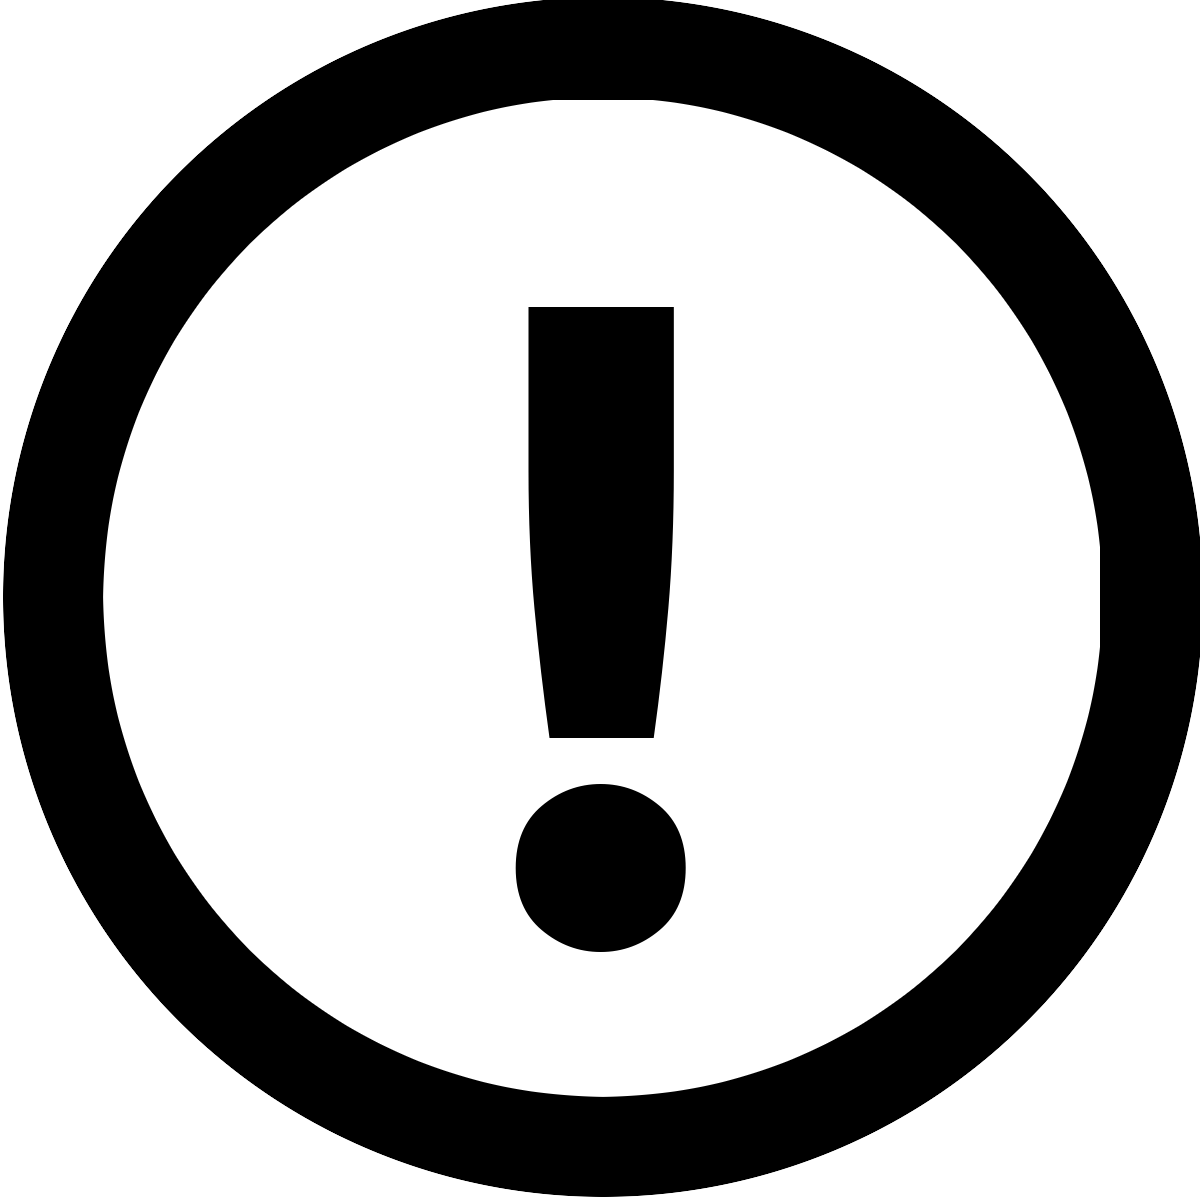
\includegraphics[width=.75\linewidth]{Bilder/recap}
            \textsc{\autoref{#1}}
            \vspace{-25pt}
        \end{wrapfigure}
        #2
        \todo[inline]{Racap!}
    \end{minipage}
}

\newcommand{\recap}[2]{
    \setlength{\fboxsep}{1.5em}
    \colorbox{gray!25}{\parbox{\linewidth-2\fboxsep}{\recappage{#1}{#2}}}
}

% sonstige Präambel
% Workaround f�r lstlistoflistings --------------------------------
\makeatletter
\@ifundefined{float@listhead}{}{%
    \renewcommand*{\lstlistoflistings}{%
        \begingroup
    	    \if@twocolumn
                \@restonecoltrue\onecolumn
            \else
                \@restonecolfalse
            \fi
            \float@listhead{\lstlistlistingname}%
            \setlength{\parskip}{\z@}%
            \setlength{\parindent}{\z@}%
            \setlength{\parfillskip}{\z@ \@plus 1fil}%
            \@starttoc{lol}%
            \if@restonecol\twocolumn\fi
        \endgroup
    }%
}
\makeatother

% Nummerierungstiefe
\setcounter{secnumdepth}{3}
\setcounter{tocdepth}{3}

% Farben
\definecolor{LightGray}{gray}{0.95}

\lstdefinelanguage{QML} 
{morekeywords={color,background,margin, visible, width, height, title, id, fill, text, anchors, centerIn, onClicked, host, onMessageReceived, Component.onCompleted, Component, onCompleted}, 
	emph={ApplicationWindow, Rectangle, Button, QmlQmqtt},
	sensitive=false, 
	morecomment=[l]{//}, 
	morecomment=[s]{/*}{*/},
	morestring=[b]", 
} 


\lstdefinelanguage{json}  
{
	emph={:, \,},
	sensitive=false, 
	morecomment=[l]{//}, 
	morecomment=[s]{/*}{*/},
	morestring=[b]", 
} 

\newcommand{\specialcell}[2][c]{%
	\begin{tabular}[#1]{@{}c@{}}#2\end{tabular}}

\titlehead{
Universität Augsburg \\ Fakultät für angewandte Informatik \\ Institute for Software \& Systems Engineering
}
\title{Programmiersprachliche Konzepte von COBOL im Vergleich mit Java -- Eine praxisorientierte Einführung}
\subject{Masterarbeit \\\normalsize{Informatik und Multimedia}}
\author{
    \Huge{Antonio Grieco} \\\\
        \small{Matrikelnummer: 1498410} \\ 
        \small{antonio.grieco@gmx.de} \\
        \small{Rosenaustraße 70} \\ 
        \small{86152 Augsburg}
} 
\publishers{
     \vfill
      Erstgutachter: Prof. Dr. Alexander  Knapp\\
      Zweitgutachter: Prof. Dr. Bernhard  Bauer
}
\date{\vfill \vfill \vfill \today}

% Das eigentliche Dokument -----------------------------------------------------
%   Der eigentliche Inhalt des Dokuments beginnt hier. Die einzelnen Seiten
%   und Kapitel werden in eigene Dateien ausgelagert und hier nur inkludiert.
% ------------------------------------------------------------------------------

\begin{document}
	
	% Deckblatt ---------------------------------
	\maketitle
	% \includepdf[pages=-]{Sonstiges/Deckblatt.pdf}

	% Seitennummerierung: R?mische Ziffern; Zur?cksetzen auf 1
	\pagenumbering{Roman}
	\setcounter{page}{1}
	
	% Ueberblick --------------------------------
		\chapter*{Zusammenfassung} \chapter*{Zusammenfassung} \addcontentsline{toc}{chapter}{Zusammenfassung}

Da die \quotes{\textbf{Co}mmon \textbf{B}usiness \textbf{O}riented \textbf{L}anguage}, kurz \mbox{COBOL} genannt, bereits Ende der 1950er Jahre entstand und daher nur wenige moderne Sprachkonzepte bietet, wird der Fokus in der Ausbildung neuer Informatiker immer mehr auf Programmiersprachen mit moderneren objektorientierten Konzepten gelegt. Dem steht gegenüber, dass COBOL immer noch wichtiger Bestandteil bestehender betrieblicher Informationssysteme ist, die es zu warten und zu erweitern gilt. Während diese Sprache heutzutage also zunehmend seltener Teil der Ausbildung von Programmierern ist, besteht, durch die Vielzahl vorhandener COBOL-Systeme, weiterhin eine hohe Nachfrage nach Experten.

Diese Arbeit gibt einen generellen Überblick über Herausforderungen, die sich in Verbindung mit betrieblichen Informationssystemen ergeben, und zeigt, wie COBOL und Java diesen Problemen begegnen. Ferner wird COBOL konzeptuell erfasst und mit Java, als Vertreter moderner Sprachen, verglichen. Dabei steht stets die praktische Anwendung der Sprachen im Vordergrund, weshalb Experteninterviews geführt wurden, um neben bestehender Fachliteratur bestmögliche Einsicht in die Entwicklung und Wartung angesprochener Systeme zu erhalten. Damit entstand ein Leitfaden, der es Programmierern mit Java-Kenntnissen erlaubt, sich mit COBOL vertraut zu machen, indem bekannte Konzepte, Muster und Konstrukte gegenübergestellt werden. Zusätzlich wird, als Ergebnis der Experteninterviews, darauf hingewiesen, wie sich der Umgang mit diesen Konzepten in der Praxis gestaltet und gestalten sollte. 
	\chapter*{Abstract} \chapter*{Abstract} \addcontentsline{toc}{chapter}{Abstract}

COBOL, which stands for the \quotes{\textbf{Co}mmon \textbf{B}usiness \textbf{O}riented \textbf{L}anguage}, began to rise in the late 1950s as a project of the US government. The aim was to design a programming language, which enables persons without knowledge of programming to engineer software systems. At that time nobody could forebode, that it's still used in many existing operational information systems and not uncommon that these have different requirements than modern desktop or web applications regarding the environment and development. So, whilst COBOL is getting less and less attention of new programmers the demand for highly trained and experienced professionals is high yet. This thesis outlines key challenges in terms of those operational information systems and reveals how COBOL copes with them. Furthermore, COBOL gets conceptually surveyed and compared with Java, which represents state of the art programming languages. The practical approach is always on focus in this comparison, and therefore, along with available literature, experts were interviewed to get the best possible insight of development and maintenance of those systems. The purpose was to devise a guide for Java developers, which enables them to familiarize with COBOL by contrasting known concepts, pattern and constructs. The interviews led to best practice advices in combination with those concept descriptions and hints on how those are used in practice and how they should be.
	
%	\singlespacing{
		\clearpage \tableofcontents					% Inhaltsverzeichnis
		\clearpage \listoffigures					% Abbildungsverzeichnis
		\clearpage \lstlistoflistings				% Quellcode-Listings
	%	\clearpage \listoftables					% Tabellenverzeichnis
	%	\clearpage \chapter*{\hypertarget{listofnomenclaturelink}{Abkürzungsverzeichnis}}
\addcontentsline{toc}{chapter}{Abkürzungsverzeichnis}


\begin{acronym}[OPC HDA ]
	\acro{AMQP}{Advanced Message Queuing Protocol}
\acro{API}{Programmierschnittstelle}
\acro{APK}{Android application package}
\acro{CEP}{Complex Event Processing}
\acro{COM}{Component Object Model}
\acro{CPS}{Cyber-physisches System}
\acro{DCOM}{Distributed COM}
\acro{DDS}{Data Distribution Service}
\acro{DSG}{Distributed Systems Group}
\acro{GCC}{GNU Compiler Collection}
\acro{GCM}{Google Cloud Messaging}
\acro{GUI}{Graphical User Interface}
\acro{HMI}{Human-Machine-Interface}
\acro{IDE}{Integrated Development Environment}
\acro{IoT}{Internet der Dinge}
\acro{JDK}{Java Development Kit}
\acro{LHS}{left-hand side}
\acro{M2M}{Maschine-zu-Maschine}
\acro{moc}{Meta-Object Compiler}
\acro{MQTT}{Message Queue Telemetry Transport}
\acro{NDK}{Native Development Kit}
\acro{OASIS}{Organization for the Advancement of Structured Information Standards}
\acro{OPC A/E}{OPC Alarms and Events}
\acro{OPC DA}{OPC Data Access}
\acro{OPC DX}{OPC Data exchange}
\acro{OPC HDA}{OPC Historical Data Access}
\acro{OPC UA}{OPC Unified Architecture}
\acro{OPC}{Open Platform Communications}
\acro{PLC}{Programmable Logic Controller}
\acro{QML}{Qt Meta-object Language}
\acro{QoS}{Quality of Service}
\acro{RHS}{right-hand side}
\acro{SCADA}{Supervisory Control and Data Acquisition}
\acro{SDK}{Software Development Kit}
\acro{SPS}{Speicherprogrammierbare Steuerung}
\acro{WSN}{Wireless Sensor Network}
\end{acronym}	% Abk?rzungsverzeichnis
%	}
	
	% Zeilenabstand setzen
	\onehalfspacing
	
	% Seitennummerierung: Speichern der Seitennumber in RomanSiteCounter; Arabische Ziffern; Zur?cksetzen auf 1
	\pagebreak
	\newcounter{RomanSiteCounter}
	\setcounter{RomanSiteCounter}{\value{page}}
	\pagenumbering{arabic}
	\setcounter{page}{1}
	
	% Inhalt ------------------------------------
		% Einleitung ----------------------------
			\chapter{Einleitung} 



\label{ch:einleitung}
    %\section{Typographische Konventionen}
In diesem Abschnitt werden typographische Konventionen festgelegt, um das Verständnis zu erleichtern.
\begin{itemize}
	
	\item	Fachbegriffe werden \Fachbegriff{kursiv} geschrieben.
	
	\item	Zitate werden in \quotes{doppelten Anführungszeichen} geschrieben.
	
	\item	Quellcode wird in \mintinline{text}{Festschrittschrift} geschrieben.
	\item	Neue und wichtige Begriffe werden \NeuerBegriff{fett} geschrieben.
	
	\item	Abkürzungen werden bei der ersten Verwendung ausgeschrieben und können zusätzlich im
			\hyperlink{listofnomenclaturelink}{Abkürzungsverzeichnis} nachgeschlagen werden.
\end{itemize}
    \section{Problemstellung}\label{problemstellung}
Der folgende Abschnitt soll die Problemstellung verdeutlichen, welche der Arbeit zu Grunde liegt. 
Dazu wird erläutert, welche Wichtigkeit COBOL genießt und anschließend mit der Bedeutung, die der Sprache in der Lehre tatsächlich beigemessen wird und den Folgen davon für den Arbeitsmarkt, gegenübergestellt.

\subsection*{Wichtigkeit von COBOL}\label{wichtigkeit}
\quotes{Viele Millionen Cobol-Programme existieren weltweit und müssen laufend gepflegt werden.
Es ist bei dieser Situation undenkbar und unter wirtschaftlichen Gesichtspunkten unvertretbar in den nächsten Jahren eine Umstellung dieser Programme auf eine andere Sprache durchzuführen.} \cite{_ist_1979}

Was Herr Dr. Strunz neben vielen anderen Experten bereits 1979 prophezeite hat auch heute noch Gültigkeit. Obwohl COBOL zum Ende der 50er Jahre entstand, 1959 veröffentlicht wurde und damit fast 60 Jahre alt ist, trifft man es auch heute noch häufig an. In der britischen Tageszeitung The Guardian, zitiert der Autor Scott Colvey in seinem Artikel %``\citefield{colvey_cobol_2009}{title}'' 
\cite{colvey_cobol_2009} anlässlich des 50. Geburtstages von COBOL den Micro Focus Manager David Stephenson: \quotes{`some 70\% to 80\% of UK plc business transactions are still based on Cobol'}. 
Weiter führt er darin Aussagen von IBM Software-Leiters Charles Chu an, welcher die Aussagen von Stephenson bestätigt: \quotes{$[\ldots]$ there are 250bn lines of Cobol code working well worldwide. Why would companies replace systems that are working well?'}. 
Stephen Kelly, Geschäftsführer von Micro Focus, betont zudem, dass sich Stand 2009 über 220 Milliarden COBOL-Codezeilen im produktiven Einsatz befanden, welche vermutlich 80\% der insgesamt weltweit aktiven Codezeilen ausmachten. Außerdem wurden damaligen Zeitpunkt wurden geschätzt 200-mal mehr COBOL-Transaktionen ausgeführt als Google Suchanfragen verzeichnen konnte. \cite{kelly_cobol_2009} Diese Aussagen decken sich mit den Angaben in \citeWithTitle{doke_cobol_2005}. Auch darin heißt es, dass mit 225 Milliarden Codezeilen, etwa 70\% des weltweiten Codes in COBOL geschrieben sind.

Nicht nur, dass COBOL in den vergangenen Jahren also einen enormen Marktanteil ausmachte wird also deutlich, sondern auch die Bedeutung für die Zukunft: Wieso sollte funktionierender Code mit Hilfe von teuren und riskanten Prozessen ersetzt werden?

Da sich viele Unternehmen der Frage eines Umstiegs von COBOL auf eine modernere Lösung ausgesetzt sehen, auf die sich nur schwer eine Antwort finden lässt, welche die Risiken und Kosten aufwiegt, stieg die Anzahl \todo[inline]{Beleg} des sich weltweit in Produktion befindlichen COBOL-Codes über die vergangen Jahre sogar noch weiter an.
Dieses Risiko ergibt sich vorrangig durch die Trasnaktion immenser Geldsummen, die mit COBOL-Systemen durchgeführt werden: \quotes{Täglich werden Transaktionen mit einem Volumen von schätzungsweise drei Billionen Dollar über Cobol-Systeme abgewickelt. Dabei geht es um Girokonten, Kartennetze, Geldautomaten und die Abwicklung von Immobilienkrediten. Weil die Banken aggressiv auf eine Digitalisierung ihres Geschäftes setzen, wird Cobol sogar noch wichtiger. Denn Apps für Smartphones etwa sind in modernen Sprachen geschrieben, müssen aber mit den alten Systemen harmonieren.} \cite{beat_balzli_cobol-programmierer_2017}

Im TIOBE-Index\cite{_tiobe_} für April 2018 rangiert COBOL auf Platz 25 mit einem Rating von 0.541\%. Dieser Index wird auf Basis von Suchanfragen nach den entsprechenden Programmiersprachen, auf den meist frequentiertesten Internetseiten, erstellt. COBOL ist somit zwar nur Teil jeder 200. Suchanfrage, rangiert jedoch damit trotzdem vor anderen etablierten oder aufstrebenden Sprachen wie \textit{Kotlin}, \textit{Scala} oder \textit{Haskell}. Außerdem gilt es hier zu beachten, dass COBOL zu einer Zeit entstand, in der das Internet noch lange nicht existierte und Informationen über die Sprache mittels Büchern verbreitet und vermittelt wurden. Daher ist auch heute noch das Internet nicht die vorrangige Quelle, um Wissen über COBOL zu akquirieren. Unter diesen Gesichtspunkten ist das TIOBE-Rating von COBOL als noch höher einzuschätzen.


\subsection*{Bedeutung in der Lehre}
Da COBOL bereits 60 Jahre alt ist haben heutzutage bereits viele einstige COBOL-Entwickler das Rentenalter erreicht. Im Artikel \citeWithTitle{beat_balzli_cobol-programmierer_2017} beschreibt der Autor exemplarisch den Fall eines 75-jährigen Entwickler, der ob seiner Erfahrung und trotz seines Alters immernoch in der Branche tätig ist.

Junge COBOL-Entwickler sind rar, da COBOL nur noch selten Teil der Ausbildung ist. \citeauthor{doke_cobol_2005} führen in \citeWithTitle{doke_cobol_2005} an, dass im Jahr 2002 lediglich in 36.2\% COBOL Teil des Gundstudiums war, obwohl im Jahr 1995 noch 89.7\% der befragten Bildungseinrichtungen angaben COBOL-Kurse als festen Bestandteil der Ausbildung zu haben. Sieht man sich dagegen die Zahlen zu Java als Vertreter moderner Programmiersprachen an, lässt sich ein klarer Trend erkennen. Erst 1995 entstanden, stieg die Zahl der  Universitäten, die Java lehrten von 42.5\% im Jahr 1998 auf 90.0\% im Jahr 2002. Spinnt man diesen Wandel ins heutige Jahr weiter, zu dem sich in der Zwischenzeit noch eine Fülle neuerer lässt sich erahnen wie selten Lehrveranstaltung zum Thema COBOL inzwischen geworden sind.

Man sieht also, dass sich die Lehrer, obwohl der Bedarf an COBOL-Programmierern weiterhin immens ist, stark weg von COBOL fokussiert hat was die Wirtschaft zusammen mit dem zunehmenden Alter erfahrener COBOL-Entwickler vor Probleme stellt.

\subsection*{Kontroverse Beurteilungen von COBOL}
Die in \autoref{wichtigkeit} angeführten Aussagen und Meinungen stammen oftmals von Personen aus dem Umfeld von Unternehmen, die teils hohen Profit aus dem Weiterbestehen COBOLs herausschlagen. Diese Aussagen sind daher, wenn auch sicherlich nicht falsch, vorsichtig und vor allem sehr differenziert zu betrachten.

Der mehrfach prämierte Informatiker \citeauthor{edsger_wybe_dijkstra_how_1975} z.B. findet sehr klare andere Worte zu COBOL: \quotes{The use of COBOL cripples the mind; its teaching should, therefore, be regarded as a criminal offence.} \cite{edsger_wybe_dijkstra_how_1975}

\citeauthor{florian_hamann_banken_2017} nennt in seinem Artikel \citeWithTitle{florian_hamann_banken_2017} die bereits erwähnte zunehmende Knappheit von Arbeitskräften auch als einen wichtigen Faktor dafür, weshalb COBOL über kurz oder lang von moderneren Systemen und Sprachen verdrängt und abgelöst wird.

Trotz dieser Kontroversen kann festgehalten werden, dass es nach wie vor eine gleichbleibend hohen Bedarf an Entwicklern gibt, den es zu decken gilt.
    \section{Ziel der Arbeit}
Die vorliegende Arbeit leistet einen Beitrag zur Lösung der in \autoref{problemstellung} beschriebenen Probleme. Dies geschieht mithilfe eines Leitfadens, der fachkundigen Java-Entwicklern den Einstieg in COBOL erleichtert, indem gängige Sprachkonzepte gegenübergestellt und verglichen werden. 

Das ermöglicht es, vorhandenes Wissen über Softwareentwicklung, im speziellen mit Java, in einen COBOL-Kontext zu bringen und passende Sprachkonzepte nutzen zu lernen. Des Weiteren wird aufgezeigt, welche konzeptuellen Herausforderungen sich bei der COBOL-Entwicklung und Migration ergeben.

Im Fokus steht hierbei neben der Einführung in relevante Sprachkonstrukte stets auch die Experteneinschätzung zur Nutzung der verschiedenen Konzepte. Daher wird, wenn möglich, zusätzlich zu den erklärten Paradigmen erläutert, wie die Verwendung in der Praxis aussehen \bzw nicht aussehen sollte und je nach Sprachmittel gegebenenfalls in der Praxis zu verwendende Alternativen aufgezeigt.

Es ist nicht Ziel der Arbeit, vorhandene Java-Entwickler zu Neuentwicklungen mit COBOL zu animieren oder diese gar zu COBOL-Entwicklern umzuschulen. Wichtig ist in diesem Zusammenhang vielmehr, ihr Wissensspektrum so zu erweitern, dass es ihnen möglich wird, komplexe fachliche Zusammenhänge, vor allem die \quotes{business logic}, bestehender COBOL-Architekturen zu erkennen und zu verstehen. Dadurch sind diese Entwickler flexibler einsetzbar und geschult, um mit Migrations-, Renovierungs- und Wartungsaufgaben von COBOL-Systemen betraut werden zu können.

Neben den praxisrelevanten Aspekten erfasst diese Arbeit Java und COBOL konzeptuell und bringt die Sprachen so in einen universitären Kontext. Dies dient dem Zweck, die zugrunde liegenden Ansätze statt deren syntaktischer Schreibweisen zu untersuchen. Außerdem werden dabei bekannte, in der Praxis häufig zu findende Muster beleuchtet und mit den zutage geförderten Kernkonzepten der Sprachen verglichen, um Aufschluss darüber zu geben, wie die Sprachkonzepte in der Praxis angewendet \bzw genutzt werden.
	\section{Aufbau der Arbeit}
		% Methodik
			\chapter{Methodik} 
\label{ch:chap1}
	\section{Vorhandene Literatur}
Die aufgeführte Literatur gibt oftmals mehr einen gesamtheitlichen Einblick in COBOL und bietet Hilfestellungen mit \quotes{Nachschlage-Charakter}. So wie in beispielsweise \citeWithTitle{budlong_teach_1997}, \citeWithTitle{university_of_limerick_department}  oder \citeWithTitle{jia_walker_cobol_2004} werden häufig viele der möglichen Konstrukte in COBOL vorgestellt, mit Beispielen beschrieben und so ihre Verwendung gezeigt. 

Neuere Literatur wie \citeWithTitle{stern_cobol_2006} betrachten dabei häufig zusätzlich Neuerungen wie die objektorientierte Verwendung von COBOL. \citeWithTitle{rozanski_cobol_2004} 
hingegen stellt mehr ein Syntax-Wörterbuch dar, als eine wirkliche Beschreibung oder Einführung in COBOL.

\citeWithTitle{coughlan_beginning_2014} bietet den wohl umfassensten Überblick, ausführliche Beispiele und Erklärungen zur Verwendung und wirkt dabei nicht wie ein klassisches Nachschlagewerk sondern wie ein klar strukturiertes Fachbuch das jedoch mit einem klaren roten Faden durch die Bestandteile von COBOL führt. Dabei zieht es vor allem in der Einführung auch an einigen wenigen Stellen Parallelen zu Java. 

Alle dieser Werke setzen ein ein gewisses generelles Vorwissen im Bereich der Programmierung und Informatik voraus, was auch in dieser Arbeit der Fall sein soll. Jedoch ist an nur wenigen Stellen ein vergleichender Charakter zu anderen Sprachen zu erkennen und sehr selten die Erwähnung der jeweiligen Praxisrelevanz oder der besten Einsatzmöglichkeiten zu finden. 

Diese Arbeit soll daher nicht die vielfältig bestehende Literatur um ein weiteres ähnliches Werk ergänzen sondern wichtige Bestandteile der Sprachen gegenüberstellen und Vorgehensweisen bei der Entwicklung aufzeigen. Dabei wird bewusst nur selten in die Tiefe der einzelnen Bestandteile eingegangen und alle möglichen Verwendungsarten beschrieben, sondern versucht praktisch relevante Aspekte zu beleuchten. Für einen tieferen Einblick in die gesamten Sprachfeinheiten bietet sich die bereits erwähnte Literatur an, welche auch bei der Erstellung der Inhalte als Informationsquelle genutzt wurde.
\todo[inline]{\citeWithTitle{byrne_java_2009}}
\todo[inline]{\citeWithTitle{doke_cobol_2005}}
	\section{Herangehensweise}\label{herangehensweise}
		% Konzeptuelle Herausforderungen -------------------------------
			\chapter{Herausforderungen für COBOL und Java in betrieblichen Informationssystemen}
Bei der Entwicklung von betrieblichen Informationssystemen sehen sich Entwickler mit grundlegenden Fragen und Anforderungen an die einzusetzenden Technologien und Programmiersprachen konfrontiert.

Dieses Kapitel gibt einen Überblick über die wichtigsten Entscheidungskriterien für die Herangehensweise und zeigt auf, welchen Herausforderungen sich Programmiersprachen -- im Speziellen COBOL und Java -- in diesen Informationssystemen stellen müssen.

\label{ch:herausforderungen}
    \section{Datenmengen und Dimensionierung}

Betriebliche Informationssysteme sind in der Regel dafür konzipiert, große Datenmengen zu verarbeiten, die \idR mit der Betriebszeit des Systems weiter zunehmen. Daher ist bereits bei der Planung wichtig, den späteren Datenumfang so abzuschätzen, dass nachträgliche Erweiterungen durch möglichst wenig Programmieraufwand zu bewerkstelligen sind.

Die Dimensionierung von Datenstrukturen nimmt in Java eine untergeordnete Rolle ein, da dynamisch Speicher alloziert werden kann, wodurch sich die Größe von Datenstrukturen dynamisch erweitern lässt, wie \autoref{datenstrukturen} genauer beschreibt. Um ein hohes Datenaufkommen in adäquater Zeit bewältigen zu können, spielt in Java neben der Algorithmik auch parallele Verarbeitung eine vorrangige Rolle. Ebenso beeinflusst oftmals die Plattform, auf der ein Java-System betrieben wird, wie sich die Performanz des Systems gestaltet.

Wenn Daten gleichzeitig im Speicher gehalten werden müssen, sind in COBOL Vorüberlegungen zur Dimensionierung eines Systems und der darin genutzten Datenstrukturen weitaus wichtiger als in Java. Da COBOL, wie später in dieser Arbeit beschrieben, keine dynamischen Datenstrukturen bietet, muss bereits zu Beginn sehr genau überdacht werden, wie viele Daten ein System später gleichzeitig be- und verarbeiten soll. Die befragten Experten gaben an, dass Wartungsaufträge teilweise lediglich damit zu tun haben, dass Datenstrukturen -- beispielsweise Arrays oder Strings -- zu klein dimensioniert sind und künftig mehr oder längere Datensätze aufnehmen sollen. Herr Streit bestätigte dies durch ein Beispiel aus der Praxis, bei dem eine vierstellige Nummer nicht mehr ausreichend war, um Partnerunternehmen zu identifizieren. \quotes{Gelöst wurde das dann [...] durch das Zulassen von Buchstaben, weil so der Speicherbedarf nicht erhöht wurde und sich Datenstrukturen im Speicher nicht verschoben haben.} Dies illustriert einen wichtigen Aspekt von Datenstrukturen in COBOL, der später genauer beleuchtet wird: Obwohl solche Anpassungen, im Gegensatz zu Java, in COBOL vorkommen, muss stets bedacht werden, wo Variablen im Speicher liegen, da andere Daten- und Dateidefinitionen von dem bestehenden Aufbau der Datenstrukturen ausgehen.
    \section{Langlebigkeit, Wartbarkeit und Verlässlichkeit} \label{verlaesslichkeit}

Durch ihre hohe Komplexität werden betriebliche Informationssysteme \idR über viele Jahre oder sogar Jahrzehnte betrieben und dabei gewartet, erweitert und angepasst. Um die Langlebigkeit, Wartbarkeit und Verlässlichkeit solcher Systeme sicherzustellen, werden diese in der Praxis mehr oder weniger umfangreichen Tests unterzogen. Damit kann beispielsweise sichergestellt werden, dass bestehender Code auch nach Erweiterungen weiterhin funktioniert. Eine der wichtigsten Techniken hierbei sind sogenannte Unit-Tests. Dabei werden einzelne isolierte Einheiten getestet und so Einflüsse von anderen Programmteilen minimiert. 

In Java gibt es einige Frameworks, beispielsweise \textit{JUnit}\footnote{\url{https://junit.org/} \visitedOn} oder \textit{Mockito}\footnote{\url{http://site.mockito.org/} \visitedOn}, die das Testen direkt oder indirekt unterstützen. Die Wartbarkeit begünstigt in Java zusätzlich das relativ einfache Durchführen von Refactorings. So können Programme mithilfe von modernen Entwicklungsumgebungen teilweise neu geschrieben \bzw strukturiert werden und bestehender Code so im Zuge von Erweiterungen verbessert werden. Auch hierbei sind Tests zur Überprüfung der Korrektheit von Vorteil. 

COBOL bietet zum Testen weitaus weniger Möglichkeiten. Entwicklung, Testen und Debuggen direkt am Host sind teuer, da die Kosten eines Mainframes oft nach Rechenzeit berechnet werden, und daher wurden, laut Herrn Lamperstorfer vor allem in frühen COBOL-Systemen, oftmals funktionierende und manuell getestete \quotes{Schablonen} beispielsweise für die Dateiverarbeitung zur Erweiterung eines Systems wiederverwendet, sodass diese nur minimal angepasst werden mussten. Auch Refactorings nehme man in COBOL-Systemen tendenziell selten vor, da diese ein umfangreiches Testen erfordern würden.

In puncto Verlässlichkeit können sich COBOL-Anwendungen jedoch oftmals auf gut isolierte Infrastrukturen verlassen, die durch ihre Homogenität, wenig Fortentwicklung und eingebaute Ausfallsicherheitsmaßnahmen eine zuverlässige Basis bieten. Java-Systeme hingegen werden auf vielen unterschiedlichen Plattformen betrieben, die sich sehr schnelllebig verändern, wodurch zusätzliches Augenmerk auf die Sicherung der oben genannten Eigenschaften gelegt werden muss.
    \section{Modularisierung, Wiederverwendbarkeit \& Variabilität}\label{wiederverwendbarkeit}
Sehr wichtige Punkte bei der Entwicklung von betrieblichen Informationssystemen sind die Modularisierung und Wiederverwendbarkeit. Um ein System für die Zukunft wart- und erweiterbar zu machen ist eine gewisse Modularisierung anzustreben. Code muss somit nicht mehrmals geschrieben werden, was auch das spätere Einarbeiten in ein Projekt erleichtert, da der Projektumfang deutlich verringert werden kann. 

Zudem ist, sei es um um Beispiel verschiedene Mandanten, Tarife oder Sparten abzubilden, die im Grunde die selbe Logik beinhalten, in betrieblichen Informationssystemen häufig eine gewisse Variabilität gefordert. Auch diese kann durch Wiederverwendbarkeit und Modularisierung stark begünstigt werden.

\subsection*{Java}
Java ist eine hoch modulare Sprache. Alleine objektorientierte Paradigmen wie Kapselung, Polymorphie oder Aggregation/Komposition sorgen dafür, dass Code in hohem Maße wiederverwendet werden kann. Dabei ist vor allem die Gliederung in Klassen und Funktionen (siehe \autoref{sec:functionsAndReturnValues}) ausschlaggebend. Des weiteren können Bibliotheken als Java Archive (kurz \mintinline{java}{jar} genannt) dis­tri­bu­ie­rt werden und in anderen Projekten wiederverwendet werden. Dieses Konzept nutzt auch die Programmiersprache an sich bereits in hohem Maße aus und so werden viele Funktionalitäten über Packages (siehe \autoref{structure}) bereitgestellt. Die am häufigsten gebrauchten Bibliotheken sind dabei \mintinline{java}{java.util}, welche grundlegende Datenstrukturen wie zum Beipiel Listen (siehe \autoref{lists}) bereitstellt, \mintinline{java}{java.io} welche Datenein- und Ausgabe ermöglicht und allen voran \mintinline{java}{java.lang} welche -- wie der Name bereits andeutet -- Ergänzungen zu Programmiersprachlichen Mitteln liefert. 

Durch diese praktischen Modularisierungsmöglichkeiten ist es in Java auch gut möglich Variabilität zu erreichen. So kann bestehende Logik wiederverwendet oder beispielsweise durch Vererbung minimal angepasst und nachträglich erweitert werden und sorgt dafür, dass Wartungen am System die sich auf Erweiterungen des Umfangs beziehen -- z.B. das Einführen eines neuen Tarifs -- mit verhältnismäßig geringem Aufwand umgesetzt werden können.

Ein weiterer Punkt der Java zu einer Sprache macht, die dafür sorgt, dass Programme wiederverwendet werden können ist die Tatsache, dass Java in plattformunabhängigen Byte-Code übersetzt wird. Die Java-Virtual-Machine (\textit{JVM}) führt dann diesen Byte-Code aus und sorgt so dafür, dass bereits kompilierte Programme auf allen Systemen mit JVM ausführbar sind und so weiterverteilt werden können ohne neu kompiliert werden zu müssen. Diese JVM wiederum ist ein plattformabhänigiges System, welches jedoch für -- nahezu -- alle gängigen Systeme und Plattformen verfügbar ist.

\subsection*{COBOL}
Im Gegensatz zu Java lässt COBOL ein Modularisierungskonzept vermissen. Wie in \autoref{sec:functionsAndReturnValues} nachzulesen ist, fehlen grundlegende Spracheigenschaften um die Wiederverwendbarkeit von Code sicherzustellen. 

Wie ein Herr Lamperstorfer betonte, sieht man daher in der Praxis oftmals Code-Blöcke die ein und die selbe Logik abbilden, aber durch die Verwendung von anderen Daten nochmals im Copy-Paste-Stil in den Code integriert wurden. Das sorgt für ein hohes Maß an Redundanz. Um diese Redundanz zu vermeiden werden aber auch gängigerweise Datenstrukturen für mehr als nur einen Zweck im Programm \quotes{missbraucht}. Darunter leidet natürlich die Les- und Wartbarkeit von COBOL-Code sehr, da häufig nicht klar ist welche Daten, in welchem Kontext, wie verwendet werden. Zu diesem Thema sei auf \autoref{affixCOBOL} verwiesen.

In COBOL kann Variabilität im Vergleich zu Java nur sehr schwer erreicht werden. Code muss oftmals in hohem Maße kopiert werden um ähnliche Funktionalität abzubilden und so fallen Anpassungen in diesem Bereich unverhältnismäßig groß aus.

Auch ein Bibliothekskonzept ist in COBOL nicht vorhanden. So werden Programme und aufgerufene Unterprogramme beim Kompilieren statisch zu einer ausführbaren Einheit gelinkt. Um dieses Verhalten zumindest soweit zu beeinflussen, dass dynamisch geladenen Unterprogramme entstehen kann als \quotes{Trick} eine Variable eingeführt werden, welche den Namen des Unterprogramms enthält. Wird nun das Programm aufgerufen, welches in dieser Variable definiert ist und nicht in einer festen Zeichkette definiert ist, nimmt der Compiler an, dass das geladene Unterprogramm variieren kann -- auch wenn der Inhalt der Variablen nicht verändert wird -- und vermeidet so ein statisches Linken.

Herr Streit merkte an dieser Stelle an, dass in der Praxis selten die Nutzung von sogenannten 

Zwar unterstützt COBOL in neueren Standards und Compilern eine objektorientierte Entwickung, jedoch ist diese Spracherweiterung in der Praxis irrelevant. Die meisten gängigen Systeme auf denen COBOL Programme betrieben werden verfügen nicht über derartig neue Compiler und auch bei der Verwendung merkt man, dass diese Konzepte nachträglich hinzugefügt wurden und eigentlich nicht Bestandteil der Sprache sind. Hat man das Glück ein System mit einem kompatiblen Compiler zu haben, so bleibt als weiterer Stolperstein der Fakt, dass die ohnehin raren COBOL-Entwickler nicht mit der Verwendung von objektorientierter Entwicklung firm sind. Daher wird diese Spracherweiterung in der vorliegenden Arbeit nicht behandelt. 
    \section{Darstellungsgenauigkeit -- Fließ- und Festkommaarithmetik}
Vorallem in betrieblichen Informationssystemen -- die oftmals Geldbeträge durch eine gewisse Anzahl von Rechenschritten errechnen sollen -- ist es unerlässlich einen Blick auf die Rechengenauigkeit des Systems und der verwendeten Sprachen zu werfen. Diese ist oftmals eine Folge der Speicherrepräsentation -- irrationale Zahlen können durch endlichen Speicherbedarf nicht abgebildet werden -- rationaler Zahlen, die erheblichen Einfluss auf den Darstellungsbereich hat. Man unterscheidet grundsätzlich zwischen Speicherungen in Fließ- und Festkomma-Darstellung.
 
\subsection*{Fließkommaarithmetik}
In modernen Programmiersprachen wie Java werden Datentypen für rationale Zahlen in der Fließkommarepräsentation gespeichert. Daher auch der Name \mintinline{java}{float} für engl. \quotes{floating point}. Diese Darstellung hat den großen Vorteil, dass sowohl kleine Zahlen die gegen Null gehen als auch sehr große Zahlen mit dem gleichen Speicherbedarf dargestellt werden können, da quasi das Dezimaltrennzeichen verschoben werden kann. Java verwendet zur Dartellung standardmäßig den Datentypen \mintinline{java}{double}, also ein \mintinline{java}{float} mit doppelter Darstellungsgenauigkeit bzw. doppeltem Speicherbedarf. Somit wird es möglich als kleinsten Absolutwert $2^{-1074}$ und als größten $(2 - 2^{-52}) \cdot 2^{1023}$ darzustellen.

Dabei werden Zahlen nach \textit{IEEE 754}-Standard in Vorzeichen, Exponent und Mantisse umgerechnet und gespeichert. Ohne näher auf diesen eingehen zu wollen sei kur erwähnt, dass dieser einen Algorithmus festlegt, mit dessen Hilfe Variablen in einem Speicherbereich repräsentiert werden. Dieser Speicherbereich kann sich je nach Datentyp und Programmiersprache zwar unterscheiden, ist jedoch an sich stets fester Größe. Dadurch und durch den Umstand, dass Zahlen vor dem Speichern umgerechnet werden ergibt sich die Problematik, dass bestimmte Zahlen nicht exakt repräsentiert werden können und lediglich die \quotes{näheste} Repräsentation gespeichert werden kann. Dieser Effekt ist schwer absehbar und kann in der Praxis zu ungenauen (Zwischen-)Ergebnissen führen.

\java{PrecisionExample.java}
\sepCodeAndOutputCheck
\begin{shellwindow}
$ javac PrecisionExample.java 
$ java PrecisionExample
0,64999997615814210000000 == 0.65 -> false
0.64999997615814208984375
0.65
\end{shellwindow}
\mintedCaption{Ungenauigkeit am Beispiel einer float-Variable}{floatJava}

\autoref{floatJava} zeigt beispielhaft wie die Repräsentation eines Wertes vom tatsächlichen abweichen kann. Durch die Weiterverwendung eines solchen, nicht-exakt repräsentierten, Wert würden sich unter Umständen Folgefehler in Berechnungen ergeben. Außerdem können wie gezeigt Gleicheitsvergleiche von Zahlen, insbesondere von Berechnungsergebnissen, dadurch fehlerbehaftet sein, weshalb Fließkommadatentypen stets auf ein Werteintervall statt auf Gleichheit geprüft werden sollten.

Diese beschriebenen Fließkommatypen werden stets zur Basis 2 berechnet und heißen daher auch binäre Fließkommatypen. In der \mintinline{java}{java.math}-Bibliothek findet sich jedoch auch ein Objekttyp \mintinline{java}{BigDecimal} welcher ein Fließkommawert zur Basis 10, also ein dezimales Fließkomma darstellt. Die Speicherung beruht in­des­sen auf zwei \mintinline{java}{Integer}-Werten, die ein unskalierten Faktor und einen Exponenten zur Skalierung darstellen. Außerdem ist dieser Typ steuerbar was die Rundung, die Exaktheit von Ergebnissen und das Verhalten bei nichtdarstellbaren Werten angeht. Mit den in \autoref{floatJava} aufgezeigten Effekten lässt sich außerdem festhalten, dass \mintinline{java}{BigDecimal}s nur über andere \mintinline{java}{BigDecimal}-Objekte oder \mintinline{java}{String}s zuverlässig instantiiert werden können. Andere Konstruktoren speichern die übergebenen Werte in primitiven Datentypen zwischen, wodurch eben diese ungewünschten Fehler in der Repräsentation wieder auftreten. \mintinline{java}{BigDecimal} bietet somit eine Möglichkeit Werte exakt abzuspeichern bzw. Kenntnis über unexakte Speicherung -- in der Regel durch Exceptions -- zu erhalten und diese zu steuern. Mit diesem Objekttypen gehen jedoch Speicher- und Laufzeit-Overheads einher die nicht vernachlässigt werden dürfen.

\subsection*{Festkommaarithmetik}
Um die angesprochenen Probleme zu umgehen verwenden manche Sprachen eine Festkommaarithmetik, um rationale Zahlen zu Speichern oder bieten zumindest Datentypen um eine derartige Speicherrepräsentation zu erreichen. 

Dabei wird im Gegensatz zu Fließkommazahlen festgelegt wieviele Stellen einer Zahl vor- bzw. nach dem Komma gespeichert werden sollen. Jede Ziffer wird dabei für sich -- je nach Implementierung durch eine bestimmte Codierung -- gespeichert und erlaubt somit absolute Genauigkeit im Werte- bzw. Darstellungsbereich. Auch ist der Umgang mit Überläufen fest definiert und führt zu konsistentem und abschätzbarem Verhalten. Ergebnisse werden stets zur Speicherung \quotes{abgeschnitten} außer man definiert explizit, dass gerundet werden soll. \autoref{decimalsInCobol} enthält Beispiele zu beiden Varianten. \mintinline{cobolfree}{PIC 9V9(2)} deklariert eine Variable mit genau einer Vor- und zwei Nachkommastellen. Damit wäre beispielsweise sichergestellt, dass alle Geldbeträge $< 10$ -- auch nach Berechnungen -- korrekt dargestellt werden können.

\cobol{PRECISION_EXAMPLE.cbl}
\sepCodeAndOutputCheck
\begin{shellwindow}
0.99
1.00
\end{shellwindow}
\mintedCaption{Dezimalzahlen in COBOL}{decimalsInCobol}

Ein weiterer Vorteil der Abbildung mit Festkomma ist die Tatsache, dass beliebig große Zahlen gespeichert werden können. Dies sorgt neben höherem Speicherbedarf, jedoch auch dafür, dass sofern Grundrechenarten für eine Ziffer implementiert sind, beliebig lange Ziffernfolgen nach dem gleichen Schema verarbeitet werden können. Die Ergebnisse werden dabei auch zeichenweise gespeichert und lassen so keine Rundungsfehler oder Fehler aufgrund von unzureichendem Speicherplatz zur Abbildung zu. Der Speicherbereich kann in COBOL jedoch zum Beispiel durch das Nutzen von \mintinline{cobolfree}{PACKED DECIMAL}s mit dem Schlüsselwort \mintinline{cobolfree}{COMP-3} hinter der \mintinline{cobolfree}{PICTURE}-Anweisung reduziert werden. Hierbei wird lediglich ein Nibble (\nicefrac{1}{2} Byte) pro Ziffer benötigt.

\recap{In betrieblichen Informationssystemen und speziell bei der Verarbeitung von Geldbeträgen, ist es also unerlässlich die Sicherheit einer exakten Darstellung von Zahlen zu haben. Während die binäre Fließkommadarstellung Speicherplatz-Vorteile und Flexibilität des Wertebereichs einer Zahl bietet, jedoch Werte unter Umständen nicht exakt repräsentieren kann, stellt Festkommaarithmetik sicher, dass Zahlen exakt und vorhersehbar repräsentiert werden. Dies wird durch erhöhten Speicherbereich und fehlende Flexibilität erkauft, ist jedoch in der Praxis oftmals unerlässlich. Eine Möglichkeit diese Sicherheit in Java zu erreichen ist das Nutzen des \mintinline{java}{BigDecimal}-Typen, der viele Nachteile und vor allem Unsicherheiten gegenüber binären Fließkommatypen aus dem Weg räumt. Jedoch führt dieser unter Umständen zu Performanz- bzw. Speichereinbußen. COBOL bietet mit Verwendung der Festkommaarithmetik bereits standardmäßig eine Darstellungssicherheit und Vorhersagbarkeit die vielen modernen Sprachen fehlt.}

% Vorallem in betrieblichen Informationssystemen, die oftmals an bestimmten Stellen Geldbeträge durch eine gewisse Anzahl von Rechenschritten errechnen sollen, ist es unerlässlich einen Blick auf die Rechengenauigkeit des Systems und der verwendeten Sprachen zu werfen.
% \subsection*{Rechengenauigkeit in Java}
% Java verwendet zur Speicherung von Fließkommazahlen, wie viele andere moderne Programmiersprachen, den \textit{IEEE 754}-Standard. Ohne näher auf diesen eingehen zu wollen, legt dieser einen Algorithmus fest, mit dessen Hilfe Variablen in einem Speicherbereich repräsentiert werden. Dieser Speicherbereich kann sich je nach Datentyp und Programmiersprache unterscheiden, ist jedoch an sich stets von fester Größe. Daher ist es nicht möglich beliebig genaue Werte abzubilden. 
% \java{PrecisionExample.java}
% \sepCodeAndOutputCheck
% \begin{shellwindow}
% $ javac PrecisionExample.java 
% $ java PrecisionExample
% Double addition: 199999.45
% Float addition: 199999.44
% BigDecimal addition: 199999.45
% \end{shellwindow}
% \mintedCaption{Addition von float und double Variablen in Java}{floatDoubleJava}
% \autoref{floatDoubleJava} zeigt das bereits anhand eines sehr einfachen Beispiels. Bereits die Addition von zwei Zahlen mit einer bzw. zwei Dezimalstellen, welche zugegebenermaßen bewusst so gewählt wurden, legt die Problematik offen. So unterscheiden sich die Ergebnisse der Berechnung je nach Datentyp, was auf die Abbildung der Zahlen im Speicher zurückzuführen ist. Um Sicherheit bei der Berechnung zu erhalten ist es stets nötig den Datentyp \mintinline{java}{BigDecimal}, mitsamt des damit verbundenen Speicher- und Laufzeit-Overheads, wie im letzten Teil des Beispiels gezeigt, zu verwenden. Wichtig hierbei ist, dass die Definition wenn möglich über den Konstruktor erfolgt, der eine String-Repräsentation eines Wertes erhält. Andere Konstruktoren wie z.B. \mintinline{java}{BigDecimal(double)} können zu Problemen führen, da der übergebene Wert durch die Speicherung als z.B. \mintinline{java}{double} bereits an Genauigkeit verlieren kann.
% \subsection*{Rechengenauigkeit in COBOL}
% Wie später in \autoref{variables} noch genauer ausgeführt ist der Entwickler und nicht die Sprache in COBOL dafür zuständig genau festzulegen, wie viele Dezimalstellen eine Variable speichern soll. Diese Eigenschaft in Verbindung mit der Speicherrepräsentation der Daten in COBOL führt zu einer praktisch absolut exakten Genauigkeit. %COBOL speichert dabei Daten im sogennanten \textit{BCD}-Code (Binary Coded Decimals) \todo[inline]{https://www.bernd-leitenberger.de/genauigkeit-von-computern.shtml -> Weitere Quelle!} ab. 
% Jedes Zeichen wird in COBOL separat gespeichert. Dies sorgt neben höherem Speicherbedarf, jedoch auch dafür, dass sofern Grundrechenarten für eine Ziffer implementiert sind, beliebig lange Ziffernfolgen nach dem gleichen Schema verarbeitet werden können. Die Ergebnisse werden dabei wieder auch zeichenweise gespeichert und lassen so keine Rundungsfehler oder Fehler aufgrund von unzureichendem Speicherplatz zur Abbildung zu.
    \section{Reporting}\label{reporting}
\todo[inline]{EVA-Prinzip mit Zitat!}
    \section{Schnittstellen und Datenquellen}\label{schnittstellenDatenquellen}

In betrieblichen Informationssystemen stellen außerdem Schnittstellen ein wichtiges Thema dar. Sowohl das Bereitstellen von standardisierten und dokumentierten Interfaces als auch das Nutzen von anderen Systemen über ihre Schnittstellen ist stets Teil aller Anwendungsfälle. 

Vor allem in der heutigen Zeit, in der Informationssysteme nicht mehr als alleinige Verarbeitungs-, Reporting- und Darstellungsschicht fungieren, sondern eingebettet in einen größeren Kontext aus verschiedensten Modulen, mobilen Applikationen und Websites funktionieren und mit diesen kommunizieren müssen, ist ein ausgereiftes Schnittstellenkonzept und die standardisierte Bereitstellung und Nutzung von Daten und Diensten unerlässlich.

Für Java sind an dieser Stelle eine Fülle an Bibliotheken erhältlich, welche Netzwerkkommunikation über verschiedenste Protokolle auf unterschiedlichen Ebenen ermöglichen. Neben diversen verfügbaren Fremdbibliotheken bietet bereits das JDK unterschiedliche Methoden zur Kommunikation mit Fremdsystemen.

Zudem ist es durch die Definition von Interfaces auch auf Klassenebene möglich, Schnittstellen zu bieten, die eine einfache Erweiterung von und Verbindungen zu Neusystemen möglich machen.

COBOL hingegen lässt an dieser Stelle einige Funktionalität vermissen. Durch das fehlende Bibliothekskonzept -- wie in \autoref{wiederverwendbarkeit} erläutert -- und das gänzliche Fehlen von Netzwerkkommunikationsmechanismen ist es in reinem COBOL nicht möglich, Netzwerkschnittstellen festzulegen, die von außen erreichbar sind, oder solche zu nutzen. 

COBOL-Systeme nutzen daher \idR Systemmodule, um Aufgaben, wie die Netzwerkkommunikation, zu erledigen, die mit reinem COBOL nicht möglich oder aufwendig sind. Außerdem erfordern diese Systeme nicht selten Anpassungen in anderen Systemen, auch wenn es nicht sinnvoll erscheint.

Auch intern kann ein COBOL-System nur bedingt Standards definieren, die zwischen unterschiedlichen Programmteilen für einheitliche Kommunikationskanäle sorgen. Daher basieren COBOL-Systeme, wie \autoref{reporting} beschreibt, auf einfachen EVA-Prinzipien. 

Mit Tools wie IBM MQ, zuvor WebSphere MQ, \footnote{\url{https://www.ibm.com/de-de/marketplace/secure-messaging}} können Systeme allerdings so verbunden werden, dass sie miteinander kommunizieren können. Laut Herrn Lamperstorfer lässt sich damit \quotes{technisch einfach} eine Verbindung zwischen Alt- und Neusystemen herstellen, diese sei jedoch fachlich und im Hinblick auf Performanz recht schwierig umzusetzen.



\mytodo{\todo[inline]{datenquellen, datenbanken}}

\mytodo{\todo[inline]{3. Batchbetrieb -> Schnittstellen (Host nicht COBOL)}}
\mytodo{\todo[inline]{Schnittstellen datenbasiert(copies). Db nicht so relevant da host sehr schnell mit Dateien. }}
		% Vergleich wichtiger Sprachkonzepte -------------------------------
			\chapter{Vergleich wichtiger Sprachkonzepte} 
\label{ch:sprachkonzepte}
    \section{Konventionen}
Im folgenden Abschnitt sollen bestimmte Konventionen dargestellt werden, die in COBOL bzw. Java gelten.

\subsection*{Groß- und Kleinschreibung}
Bei der Programmierung behilft man sich oftmals der Groß- und Kleinschreibung, um ein höheres Maß an Struktur und Lesbarkeit des Codes zu erreichen. 

Wichtig ist hierbei vorneweg zu beachten, dass Java \quotes{case-sensitive} ist, also zwischen Groß- und Kleinbuchstaben unterscheidet, während COBOL \quotes{case-insensitive} ist, also -- außer in Strings -- keinen Unterschied macht.

In Java ist es üblich Methodennamen und veränderbare Variablen mit einem kleinen Buchstaben beginnend zu benennen. Besteht der Name aus mehreren Wörtern so wird dieser im \quotes{camel-case} geschrieben. Das heißt, dass stets Großbuchstaben für den Beginn eines neuen Wortes verwendet werden. Beispiele hierfür wären \mintinline{java}{getAdditionalData()} oder \mintinline{java}{int currentAmountOfMoney}. Klassennamen werden in dem selben Muster geschrieben, beginnen jedoch mit einem Großbuchstaben: \mintinline{java}{ToolBox}. Zu guter letzt sollten konstante Variablen und Werte innerhalb eines Aufzählungstyps durchgehend aus Großbuchstaben bestehen, wobei einzelne Wörter mit einem Unterstrich voneinander getrennt werden (\mintinline{java}{final int MULIPLY_FACTOR = 2}). \todo{COBOL}

\subsection*{Affixe}
Ein weiteres wichtiges Werkzeug bei der Strukturierung von Programmcode ist das Versehen mit Affixen (Prä- oder Suffixen).

In Java ist es hierbei nicht ratsam Affixe zu verwenden. Da diese jedoch in einigen bestehende Codebasen Verwendung finden, werden an dieser Stelle die üblichsten behandelt.

Oftmals werden Interfaces in Java mit einem vorangestellten \quotes{I} gekennzeichnet. Diese Konvention sorgt jedoch dafür, dass Implementierungen eines Interfaces namentlich nicht immer klar abgegrenzt und definiert sind. Wird beispielsweise ein Interface \mintinline{java}{IOutput} definiert so könnten valide Implementierungen \mintinline{java}{ConsoleOutput} oder \mintinline{java}{Printer-Output} sein. Jedoch erlaubt dies namentlich auch die Interface-Implementierung namens \mintinline{java}{Output}, bei der nicht ausreichend klar ist was der Zweck dieser Klasse ist.

Ein weiterer Codingstil der gelegentlich angewendet wird ist das Nutzen von \quotes{m} und \quotes{s} als Präfix von Variablen. Diese sollen kennzeichnen, dass eine Variable entweder Instanzvariable (\textbf{m}ember) oder statisch (\textbf{s}tatic) ist. Durch die Verwendung von modernen IDEs, die beide farblich unterschiedlich darstellen, und des Schlüsselwortes \mintinline{java}{this}, welches exakt für Referenzen auf Instanzvariablen gedacht ist, werden Variablen jedoch bereits ausreichend gekennzeichnet, sodass der Code durch die Verwendung dieser Präfixe unnötigerweise schwerer lesbar gemacht wird.


\todo{Ein Statement pro zeile, einrückung}
	\section{Programmablauf und Kontrollfluß}
Durch die in \autoref{sec:functionsAndReturnValues} erläuterten Unterschiede ergeben sich auch im Programmablauf Diskrepanzen. Während Java einen definierten Einstiegspunkt in ein Programm hat (\mintinline{java}{main}-Methode) wird ein COBOL-Programm stets sequenziell von oben nach unten abgearbeitet und durchlaufen. Diese Abarbeitung beginnt am Anfang der \mintinline{cobolfree}{PROCEDURE DIVISION}.\\

\subsection*{Programmablauf in Java}

\java{MainMethod.java}
\sepCodeAndOutputCheck
\begin{shellwindow}
$ javac MainMethod.java 
$ java MainMethod
Running main method!
Running other method!
Continue main method!
\end{shellwindow}
\mintedCaption{Java main-Methode}{javaMainMethod}

\autoref{javaMainMethod} demonstriert einen sehr simplen Programmablauf in Java. Wie bereits erwähnt ist der Startpunkt eines jeden Java-Programms die \mintinline{java}{main}-Methode. Von dieser aus können weitere Methoden aufgerufen werden und sobald das Ende dieser Methode erreicht ist terminiert das Programm. Im vorliegenden Beispiel wird also nach einer Ausgabe in \mintinline{java}{main}, die Funktion \mintinline{java}{otherMethod} aufgerufen, bevor der Ablauf wieder in der \mintinline{java}{main}-Methode fortgesetzt wird. Daran soll folgendes Verhalten deutlich werden: Endet eine aufgerufene Funktion wie geplant -- d.h. ohne eine \mintinline{java}{Exception} \todo{reference exception section} -- wird stets mit der nächsten Anweisung nach dem Funktionsaufruf fortgefahren.\\

Weitere Schlüsselwörter die den Kontrollfluß steuern können sind außerdem \mintinline{java}{break}, \mintinline{java}{continue} und \mintinline{java}{goto}. Zu beachten ist dabei, dass das \mintinline{java}{goto}-Schlüsselwort zwar im Sprachstandard noch definiert ist, jedoch in keiner gängigen JVM implementiert ist. Die Verwendung führt zu Fehlern beim Kompilieren. In \autoref{javaBreakContinue} finden sich beispielhafte Verwendungen der beiden anderen Schlüsselwörter.

\java{BreakContinueExample.java}
\sepCodeAndOutputCheck
\begin{shellwindow}
$ javac BreakContinueExample.java 
$ java BreakContinueExample
== break example == 
(0)(1)
== continue example == 
(0)(1)(2)(8)(9)
\end{shellwindow}
\mintedCaption{Beispiele für die Verwendung von break und continue in Java}{javaBreakContinue}

Ein einfaches \mintinline{java}{break} sorgt wie gezeigt dafür, dass die direkt umfassende Schleife verlassen wird. Auch ein simples \mintinline{java}{continue} hat Auswirkungen auf die direkt beinhaltende Schleife. So sorgt es dafür, dass der aktuelle Schleifendurchlauf abgebrochen und mit dem nächsten fortgefahren wird. \autoref{mehrfachverzweigungen} zeigt eine weitere Verwendung des \mintinline{java}{break}-Statements.

\java{BreakContinueLabelExample.java}
\sepCodeAndOutputCheck
\begin{shellwindow}
$ javac BreakContinueLabelExample.java 
$ java BreakContinueLabelExample
== break label example == 
(0 0)(0 1)(0 2)
== continue label example == 
(0 0)(0 1)(0 2)(1 0)(1 1)(1 2)(2 0)(2 1)(2 2)
\end{shellwindow}
\mintedCaption{Verwendung von break und continue mit Label in Java}{javaBreakContinueLabel}

Deutlich unüblicher -- jedoch nicht weniger relevanter -- ist der Gebrauch eines Labels in Java. Dieses Label kann in der Verbindung mit einer \mintinline{java}{break}- oder \mintinline{java}{continue}-Anweisung genutzt werden, um mehrere umfassende Schleifen verlassen bzw. um mit dem nächsten Schleifendurchlauf einer weiter außen befindlichen Schleife fortgefahren zu werden. Die Anweisung betrifft dabei die Schleife, welche das Label trägt. Dies zeigt \autoref{javaBreakContinueLabel}.

\subsection*{Programmablauf in COBOL}

In COBOL gestaltet sich der Programmablauf gänzlich anders. Das Programm wird stets von oben nach unten durchlaufen. Wobei dieser lineare Ablauf durch die Verwendung von \mintinline{cobolfree}{PERFORM}-, \mintinline{cobolfree}{CALL}- und \mintinline{cobolfree}{GO TO}-Anweisungen verändert werden kann. An dieser Stelle sei ausdrücklich erwähnt, dass die Verwendung des \mintinline{cobolfree}{GO TO}\index{GO TO}-Befehls unter allen Umständen unerlassen werden sollte, da ansonsten sehr schwer verständlicher und wartbarer Code entsteht! Die Ausführung eines COBOL-Programms endet beim Erreichen einer \mintinline{cobolfree}{STOP RUN}-Anweisung oder mit dem Ende des Programms (\mintinline{cobolfree}{END PROGRAM}).\\

\cobol{simpleControlFlow.cbl}
\sepCodeAndOutputCheck
\begin{shellwindow}
$ ./simpleControlFlow 
Main paragraph
Enter some number: 0
Main paragraph again
$ ./simpleControlFlow 
Main paragraph
Enter some number: 1 
Main paragraph again
Enter some number: 2
\end{shellwindow}
\mintedCaption{Programmablauf in COBOL}{simpleControlFlowCobol}

Die beiden Ausführungen von \autoref{simpleControlFlowCobol} zeigen das angesprochene Verhalten eines COBOL-Programms. Beim ersten Durchlauf wird für die Variable \mintinline{cobolfree}{INPUT-NUMBER} der Wert 0 eingegeben, was durch das Ausführen der \mintinline{cobolfree}{STOP RUN}-Anweisung in Zeile 15, das Beenden des Programmes bewirkt. Beim zweiten Mal wird hingegen der Wert 1 eingegeben. Dieser Wert verhindert das Abschließen des Programms in Zeile 15, wodurch der Programmablauf in Zeile 17 fortgesetzt wird und somit erneut die Eingabeaufforderung erscheint.\\

Wie in \autoref{sec:scope} beschrieben besteht ein COBOL-Programm aus verschiedenen strukturellen Komponenten. Diese haben auch einen gewissen Einfluss auf den Programmablauf. Dies soll das Beispiel in \autoref{paragraphSecionControlFlowCobol} veranschaulichen.\\

\cobol{paragraphSecionControlFlow.cbl}
\sepCodeAndOutputCheck
\begin{shellwindow}
$ ./paragraphSecionControlFlow 
Calling section:
123 
Calling paragraphs with PERFORM THRU:
123 
Calling paragraph:
1
\end{shellwindow}
\mintedCaption{Programmablaufunterschiede in COBOL mit Sections und Paragraphs}{paragraphSecionControlFlowCobol}

Wird mittels \mintinline{cobolfree}{PERFORM} eine \mintinline{cobolfree}{SECTION} aufgerufen, so werden alle Paragraphs innerhalb dieser \mintinline{cobolfree}{SECTION} der Reihe nach ausgeführt. Ruft man jedoch einen Paragraph auf, so wird nur dieser Paragraph ausgeführt. Eine weitere Möglichkeit ist die Kombination des \mintinline{cobolfree}{PERFORM} mit dem \mintinline{cobolfree}{THRU}-Schlüsselwort. Hierbei werden alle Paragraphs zwischen zwei festgelegten Paragraphs ausgeführt. Der Kontrollfluss geht bei jeder Variante stets an das Statement nach dem \mintinline{cobolfree}{PERFORM}. \todo{EXIT-Statement?}\\

Um Verwirrungen vorzubeugen und lesbaren Code zu erhalten sollten alle Paragraphs stets Teil einer \mintinline{cobolfree}{SECTION} sein und auch nur diese Ziel einer \mintinline{cobolfree}{PERFORM}-Anweisung sein. Der letzte Paragraph einer \mintinline{cobolfree}{SECTION} sollte dabei immer ein \mintinline{cobolfree}{EXIT}-Paragraph sein, also nur das Schlüsselwort \mintinline{cobolfree}{EXIT} beinhalten. So ist das Ende einer \mintinline{cobolfree}{SECTION} beim lesen des Codes klar erkennbar. Dieses Vorgehen wurde auch von \citeauthor{richards_enhancing_1984} bereits \citeyear{richards_enhancing_1984} als best-practice beschrieben  \cite{richards_enhancing_1984}.

Die meisten Code-Beispiele dieser Arbeit enthalten bewusst keinen separaten \mintinline{cobolfree}{EXIT}-Paragraph, um den Umfang und die Übersichtlichkeit der Listings so gering wie möglich zu halten. 
    \section{Deklaration von Variablen und Datentypen} \label{variables}
Eine wichtiges Sprachmittel von Programmiersprachen ist die Verwendungsmöglichkeit von Variablen. Je nach Programmiersprache haben diese Variablen unterschiedliche Eigenschaften und werden verschieden deklariert, initialisiert bzw. definiert. Dieser Abschnitt soll die Unterschiede dabei zwischen COBOL und Java herausarbeiten.\\

\subsection*{Variablen in Java}
Eine Variable in Java hat stets einen bestimmten Datentypen. Dies können primitive Datentypen wie z.B. \mintinline{java}{int} oder \mintinline{java}{double}, aber auch komplexe Objekttypen sein.\\

\mintedJava{VariableExample.java}{Variablendeklarationen in Java}{variablesJava}

Dabei werden in \autoref{variablesJava} einige Konzepte deutlich gemacht:\\
\begin{itemize}
 \item Variablen können wie in \autoref{sec:scope} sowohl als Teil einer Klasse als auch lokal innerhalb einer Methode deklariert werden. 
 \item Die Deklaration erfolg nach dem Muster \quotes{<Datentyp> <Variablenname>}.
 \item Die Initialisierung einer Variable geschieht durch das zuweisen eines Wertes.
 \item Komplexe Objekttypen können den Wert \mintinline{java}{null} haben. Das bedeutet, die Variable, die in diesem Fall eine Referenz auf einen Speicherbereich darstellt, ist leer. Hier gilt es zu beachten, dass primitive Datentypen nicht \mintinline{java}{null} sein können.
 \item Instanzen eines Objekttypen werden durch das Schlüsselwort \mintinline{java}{new} und den Aufruf eines Konstruktors erzeugt. Primitive Datentypen haben keine Konstruktoren.
\end{itemize}

Die Deklarierung einer Variable eines bestimmten Datentyps sorgt dafür, dass ausreichend Speicherplatz für diese reserviert wird. Die Stelle der Deklaration im Code ist dabei frei wählbar und muss lediglich vor der ersten Verwendung stehen.\\

\subsection*{Variablen in COBOL}
Die Deklaration von Variablen unterscheidet sich in COBOL stark von der in Java. Neben der Eigenschaft, dass Variablen nur innerhalb der \mintinline{cobolfree}{DATA DIVISION} deklariert werden können, ist in COBOL nicht die Definition eines Datentyps möglich sondern die Festlegung einer Repräsentation. \\

Dies sorgt dafür, dass bereits an der Stelle der Variablendeklaration festgelegt werden muss, wie diese Daten im folgenden Programm dargestellt werden. Das Schlüsselwort dafür ist die \mintinline{cobolfree}{PICTURE}- oder kurz \mintinline{cobolfree}{PIC}-Anweisung.\\

\cobol{variable_declaration.cbl}
\sepCodeAndOutputCheck
\begin{shellwindow}
$ ./variableExample
Mustermann 178
Mustermann
178
1.78
\end{shellwindow}
\mintedCaption{Variablendeklarationen in COBOL}{variablesCobol}

\autoref{variablesCobol} demonstriert die Deklaration von vier Variablen. Variablen Anhand dieses Beispiels sollen wiederum verschiedene Konzepte der Variablendeklaration in COBOL illustriert werden\\

Jede Variablendeklaration beginnt mit einer Stufennummer. Diese Stufennummer sorgt für Gruppierung von Variablen. Zulässig sind dabei Zahlen zwischen \textit{01} und \textit{49}. Die Stufennummern sollten mit ausreichendem Abstand gewählt werden -- in der Praxis werden dazu 5er-Schritte gewählt --  um ein nachträgliches Einfügen zwischen zwei Stufennummern zu erleichtern. Die speziellen Stufennummern \textit{66}, \textit{77} und \textit{88} werden später separat behandelt. Wie das Beispiel zeigt, lassen sich auf einzelne Variablen auch über den Gruppennamen zugreifen. \\

Der Stufennummer folgt ein eindeutiger Name für die Variable. An dieser Stelle kann jedoch auch das Schlüsselwort \mintinline{cobolfree}{FILLER} verwendet werden. Dies sorgt dafür, dass eine Platzhaltervariable angelegt wird, auf die jedoch später nicht direkt zugegriffen werden kann.\\

Die Festlegung der Repräsentation geschieht wie bereits erwähnt durch ein \mintinline{cobolfree}{PIC}. Nach diesem \mintinline{cobolfree}{PIC} wird festgelegt wie diese Variable dargestellt werden soll. \quotes{X} steht dabei für ein alphanumerisches, \quotes{9} für ein numerisches Zeichen und \quotes{A} für einen Buchstaben. Die Angabe der Stellen einer Variable wird durch die Wiederholung des jeweiligen Zeichens oder die verkürzte Notation mit der nachgestellten Anzahl der Wiederholungen in runden Klammern -- z.B. XXXX $\equiv$ X(4) -- erreicht. Als Dezimaltrennzeichen wird wie gezeigt ein \quotes{V} verwendet und ein vorangestelltes \quotes{S} sorgt dafür, dass eine numerische Variable ein Vorzeichen führt. Es wird also genau festgelegt wie viele Vor- und Nachkommastellen eine Variable hat.\\

Die Initialisierung einer Variable erfolgt durch die \mintinline{cobolfree}{VALUE}-Anweisung gefolgt von dem Wert, welcher der Variablen zugewiesen werden soll. Dabei gibt es die Schlüsselwörter \mintinline{cobolfree}{SPACE} bzw. \mintinline{cobolfree}{SPACES} und \mintinline{cobolfree}{ZERO} bzw. \mintinline{cobolfree}{ZEROS}, die anstelle eines Wertes verwendet werden können, um eine Variable mit Leerzeichen bzw. Nullen zu initialisieren.\\

Durch die Definition der Repräsentation findet man in der Praxis oft Variablen, die auf den selben Speicherbereich wie eine andere Verweisen, jedoch die dort enthaltenen Daten anders darstellen bzw. interpretieren. Dies geschieht wie im Beispiel gezeigt mithilfe des Schlüsselworts \mintinline{cobolfree}{REDEFINES}.\\

Typsicherheit ist in COBOL nicht ausreichend gewährleistet. So kann eine Variable mit \mintinline{cobolfree}{REDEFINES} oder eine Variable, welche die eigentliche gruppiert, den Speicherbereich einer anderen mit, unter Umständen völlig \quotes{falschen}, Werten befüllen. Auch sind uninitialisierte Variablen teilweise mit falschen Datentypen vorbelegt. So kann z.B. eine numerische Variable anfangs voll mit Leerzeichen sein.\\

Weitere mögliche Bestandteile dieser Deklaration werden an den entsprechenden Stellen dieser Arbeit erläutert.\\

Zum Abschluss dieses Abschnitts sei erwähnt, dass der Speicherplatz von Variablen weder in COBOL noch in Java händisch freigegeben werden. In Java sorgt der \textit{garbage collector} dafür, dass Speicherbereich, der nicht mehr verwendet wird wieder freigegeben wird. In COBOL geschieht dies mit dem Ende eines Programms.\\
    \section{Programmstruktur}\label{sec:scope}
Dieser Abschnitt behandelt die strukturellen Unterschiede von Java- und COBOL-Programmen. Dazu wird auf den Scope von Variablen eingegangen und erläutert in welche Einheiten sich die Programme der jeweiligen Sprache aufteilen lassen. Der sog. Scope, zu deutsch Gültigkeitsbereich, gibt in der Programmierung an, in welchem Bereich eine Variable gültig ist.\\ \todo[inline]{Enum und Interfaces beschreiben}
\subsection*{Java}

\subsubsection*{Scope}
In Java ist der Scope einer Variablen meist einfach zu erkennen. Eine Variable ist innerhalb der geschweiften Klammern gültig, die die Variablendeklaration beinhalten. Dies verdeutlicht \autoref{javaScope}.\\

Die Variable \mintinline{java}{memberVariable} ist innerhalb der gesamten Klasse \mintinline{java}{ScopeExample}, also in jeder enthaltenen Methode, verschachtelten Klassen und wiederum deren Methoden, gültig. Eine Variable mit selbem Namen kann auch innerhalb einer Methode deklariert werden. Auf die Instanzvariable kann mit dem \mintinline{java}{this}-Schlüsselwort zugegriffen werden. In geschachtelten Klassen muss zusätzlich der Klassenname vorangestellt werden wie Zeile 27 zeigt.  Ist keine lokale Variable mit selbem Namen vorhanden, so kann dieses Schlüsselwort auch weggelassen werden. \\

Wie Zeile 19 zeigt ist es auch nicht möglich auf lokale Variablen einer anderen Funktion zuzugreifen. Gleiches gilt für Instanzvariablen verschachtelter Klassen.\\

\mintedJava{ScopeExample.java}{Variablendeklarationen mit verschiedenen Scopes}{javaScope}

\subsubsection*{Struktur} \label{javaStructureSubsubsection}

Auch zeigt das Beispiel in \autoref{javaScope} die wichtigsten Konzepte der Strukturierung von Java-Code. Zeile 1 beinhaltet die Package-Deklaration, d.h. hiermit wird die Klasse dem hier genannten Package zugeordnet. Diese Deklaration \textbf{muss} gleich der Ordnerhierarchie sein, in denen die Java-Dateien verwaltet werden. \\

Die nächstkleinere Einheit eines Java-Programms stellen Klassen dar. Hierbei handelt es sich um das Kernkonzept der objektorientierten Programmierung. Von dieser Klasse können fortan Objekte instanziiert werden. Um einen tieferen Einblick in die Thematik der Objektorientierung zu erhalten sei an dieser Stelle einschlägige Fachliteratur erwähnt. Diese erwähnte Klasse muss dabei in einer Datei gespeichert sein, die den selben Namen trägt wie die Klasse selbst. Aus dem Klassennamen \mintinline{java}{MasterThesis} folgt also der Dateiname \mintinline{text}{MasterThesis.java}.\\

Teil dieser Klassen können wiederum Methoden, Variablendeklarationen und weitere Klassen sein. Diese können jeweils statisch oder auch einer Instanz zugeordnet sein. Auch dabei handelt es sich um ein gängiges Konzept der objektorientierten Softwareentwicklung. Hierzu sei an dieser stelle lediglich erwähnt, dass statische Methoden, Variablen und Klassen Teil der Klasse sind und kein konkret instanziiertes Objekt benötigen während nicht-statische Komponenten stets ein konkretes Objekt einer Klasse benötigen.\\

Diese weiteren Klassen haben strukturell die selben Eigenschaften wie die umgebende Klasse, außer, dass sie nicht in einer Datei gespeichert sein müssen bzw. können deren Name dem Klassennamen entspricht.\\

\begin{figure}[H]
    \centering
    \begin{tikzpicture}[node distance=0cm]
        \node (programRect) [inner sep=0pt, rectangle, draw, rounded corners, ultra thick, draw=black, fill=javaProgramm, minimum width=\textwidth, minimum height=.6\textwidth] at (0,0) {};
        \node[below = of programRect.north] () {Java Programm};
        \node (packageRect) [inner sep=0pt, rectangle, draw, rounded corners, ultra thick, draw=black, fill=javaPackage!50!white, minimum width=.9\textwidth, minimum height=.5\textwidth] at (0,0) {};
        \node[below = of packageRect.north] () {Packages};
        \node (classRect) [inner sep=0pt, rectangle, draw, rounded corners, ultra thick, draw=black, fill=javaClass!50!white, minimum width=.8\textwidth, minimum height=.4\textwidth] at (0,0) {};
        \node[below = of classRect.north] () {Klassen};
        \node (methodRect) [inner sep=0pt, rectangle, draw, rounded corners, ultra thick, draw=black, fill=javaMethod!50!white, minimum width=.325\textwidth, minimum height=.3\textwidth] at (.15\textwidth,0) {};
        \node[below = of methodRect.north] () {Methoden};
        \node (innerClassRect) [inner sep=0pt, rectangle, draw, rounded corners, ultra thick, draw=black, fill=javaClass!30!white, minimum width=.325\textwidth, minimum height=.067\textwidth] at (-.2\textwidth,.1\textwidth) {};
        \node[below = of innerClassRect.north] () {Geschachtelte Klassen};
        \node (statementRect) [inner sep=0pt, rectangle, draw, rounded corners, ultra thick, draw=black, fill=javaStatement!60!white, minimum width=.35\textwidth, minimum height=.133\textwidth] at (.15\textwidth,-.05\textwidth) {};
        \node[below = of statementRect.north] () {Statement};
        \node (variableRect) [inner sep=0pt, rectangle, draw, rounded corners, ultra thick, draw=black, fill=javaStatement!70!white, minimum width=.35\textwidth, minimum height=.133\textwidth] at (-.15\textwidth,-.05\textwidth) {};
        \node[below = of variableRect.north] () {Variablendeklaration};
        \node (anonClassRect) [inner sep=0pt, rectangle, draw, rounded corners, ultra thick, draw=black, fill=javaAnonClass!70!white, minimum width=.325\textwidth, minimum height=.067\textwidth] at (0,-.05\textwidth) {};
        \node[below = of anonClassRect.north] () {Anonyme Klasse};
    \end{tikzpicture}
    \todo[inline]{Align diagram components right}
    \caption{Strukturelle Bestandteile eines Java-Programms}
    \label{javaStructureDiagram}
\end{figure}

Methoden wiederum bestehen aus einzelnen Statements. Zu erwähnen ist, dass Variablendeklarationen auch ein Statement darstellen, jedoch sind, als Teil einer Klasse, keine anderen Statements als Variablendeklarationen gültig, weshalb auch an dieser Stelle diese Unterscheidung getroffen wird. Statements die aus Variablendeklarationen, Zuweisungen oder Methodenaufrufen bestehen, müssen im Gegensatz zu Block-Statements, wie z.B. \mintinline{java}{if}-Statements, stets mit einem Semikolon beendet werden. \\

\mintedJava{AnonymousClassAndMethodExample.java}{Anonyme Klassen und Funktion in Java}{anonymousJava}

Die letzten strukturellen Elemente sind anonyme Klassen und Funktionen, auch Lambda-Funktionen genannt. Wobei anonyme Funktionen in Java genaugenommen nur eine syntaktische Schreibweise einer speziellen anonymen Klasse sind. Die Verwendung wird in \autoref{anonymousJava} illustriert. Die Zeilen \till{9}{14} beinhalten eine anonyme Klasse, die das \mintinline{java}{IntConsumer}-Interface implementiert. Die völlig identische  anonyme Klasse wird implizit durch die Lambda-Funktion in den Zeilen \till{16}{18} implementiert.\\

\autoref{javaStructureDiagram} gibt einen zusammenfassenden Überblick über die erwähnten Teile eines Java-Programms und bildet nochmals graphisch ab, wie sich die jeweiligen Komponenten zusammensetzen können.\\

\subsection*{COBOL}
\todo[inline]{Darstellung überarbeiten}
{

\begin{wrapfigure}{l}{.5\textwidth}
\centering
    \begin{tikzpicture}[node distance=0cm]
        \node (programRect) [inner sep=0pt, rectangle, draw, rounded corners, ultra thick, draw=black, fill=javaProgramm, minimum width=\linewidth, minimum height=.6\linewidth] at (0,0) {};
        \node[below = of programRect.north] () {COBOL Programm};

        \node (divisionRect) [inner sep=0pt, rectangle, draw, rounded corners, ultra thick, draw=black, fill=javaPackage!50!white, minimum width=.9\linewidth, minimum height=.5\linewidth] at (0,0) {};
        \node[below = of divisionRect.north] () {Divisions};

        \node (sectionRect) [inner sep=0pt, rectangle, draw, rounded corners, ultra thick, draw=black, fill=javaClass!50!white, minimum width=.5\linewidth, minimum height=.4\linewidth] at (-.15\linewidth,0) {};
        \node[below = of sectionRect.north] () {Sections};

        \node (paragraphRect) [inner sep=0pt, rectangle, draw, rounded corners, ultra thick, draw=black, fill=javaMethod!50!white, minimum width=.5\linewidth, minimum height=.3\linewidth] at (.15\linewidth,0) {};
        \node[below = of paragraphRect.north] () {Paragraphs};

        \node (sentenceRect) [inner sep=0pt, rectangle, draw, rounded corners, ultra thick, draw=black, fill=javaStatement!60!white, minimum width=.4\linewidth, minimum height=.2\linewidth] at (0,0) {};
        \node[below = of sentenceRect.north] () {Sentences};

        \node (statementRect) [inner sep=0pt, rectangle, draw, rounded corners, ultra thick, draw=black, fill=javaAnonClass!70!white, minimum width=.3\linewidth, minimum height=.1\linewidth] at (0,0) {};
        \node[below = of statementRect.north] () {Statements};

    \end{tikzpicture}
\caption{Strukturelle Bestandteile eines COBOL-Programms\label{cobolStructureDiagram}}
\end{wrapfigure}
Nebenstehende \autoref{cobolStructureDiagram} zeigt die strukturellen Bestandteile eines COBOL-Programms. 

Dabei gibt es folgende vier fest definierte \mintinline{cobolfree}{DIVISION}s:
\begin{itemize}
    \item \mintinline{cobolfree}{IDENTIFICATION DIVISION}\\
    Hier werden grundlegende Daten zum Programm, wie der Name oder der Autor festgelegt.
    \item \mintinline{cobolfree}{ENVIRONMENT DIVISION}\\
    Definiert die Ein- und Ausgabe sowie Konfigurationen der Systemumgebung.
    \item \mintinline{cobolfree}{DATA DIVISION}\\
    Diese \mintinline{cobolfree}{DIVISION} beinhaltet die Definitionen von Daten. Dazu zählen Variablen oder auch Datei-Record-Definitionen.
    \item \mintinline{cobolfree}{PROCEDURE DIVISION}\\
    Innerhalb dieser \mintinline{cobolfree}{DIVISION} befindet sich der ausführbare Code.
\end{itemize}

\todo[inline]{DIVISIONS, SECTIONS, PARAGRAPHS, SENTENCES, STATEMENTS -> TERMINATED WITH DOT.}

}

\todo[inline]{Einteilung einer Zeile. Erste X Zeichen reserviert usw. 80 Zeichen länge....}

\todo[inline]{Variablen sind immer global in COBOL}
    \section{Datenstrukturen}

\subsection{Felder}
OCCURES \& Arrays

\subsection{Java List}

\subsection{Java Set}

\subsection{Java Map}
    \section{Arrays}\label{sec:felder}
Eine zentrale Datenstruktur in der Programmierung stellen Felder bzw. Arrays -- in COBOL auch als \textit{table} bezeichnet -- dar. Dabei handelt es sich um eine geordnete Sammlung von Werten eines Typs, auf die, im Gegensatz zu \zB verketteten Listen, direkt zugegriffen werden kann. 

\mintedJava{Arrays.java}{Felder in Java}{arraysJava}
Zeile 4 in \autoref{arraysJava} beschreibt das Anlegen eines Arrays in Java mittels \jav{new}-Schlüs"-sel"-wort, wohingegen Zeile 8 den Zugriff auf ein Element zeigt. Die Indizierung der Elemente beginnt dabei mit dem Element 0. Ein Feld der Größe 10 hat also die Indizes \till{0}{9}. Sowohl beim Anlegen als auch beim Zugreifen auf ein Element des Arrays wird der \jav{[]}-Operator verwendet.

In COBOL können Felder durch \cob{OCCURS}, gefolgt von der Anzahl der zu speichernden Werte und \cob{TIMES} angelegt werden. Dies illustriert \autoref{arraysCobol}. Das \cob{INDEXED BY}-Schlüsselwort kann dazu genutzt werden, eine Variable zu definieren, mit der das Array indiziert werden kann. Dies ist jedoch nicht zwangsläufig notwendig. In COBOL werden Indizes auch \textit{subscipts} genannt.

\mintedCobol{arrays.cbl}{Felder in COBOL}{arraysCobol}
In Zeile 12 ist der Zugriff auf ein einzelnes Feld-Element zu sehen. Dies geschieht in COBOL mittels runder Klammern. Zu beachten ist hierbei, dass COBOL die einzelnen Elemente beginnend mit 1 indiziert. Im Gegensatz zu Java hat ein Array der Größe 10 in COBOL also die Indizes \till{1}{10}.

Eine Besonderheit von Feldern in COBOL und in Java ist, dass diese auch mehrdimensional sein können. In COBOL spricht man statt von Dimensionen von Levels. Jedes Element der ersten Dimension bzw. des ersten Levels besteht also aus einem weiteren Feld. Ein Zugriff auf ein beispielhaftes zweidimensionales Array ist dann mittels \jav{[][]} in Java bzw. \cob{(X,Y)} in COBOL möglich. Dabei ist auch ein Zugriff auf eine ganze Dimension möglich.

Eine weitere Gemeinsamkeit ist die Tatsache, dass Felder in beiden Sprachen eine feste Größe haben. Nach dem Anlegen des Feldes kann diese Größe nicht mehr geändert werden. Jedoch muss in COBOL bereits zur Zeit der Kompilierung festgelegt werden, wie viele Elemente ein Array beinhalten soll. In Java kann diese Größe auch variabel zur Laufzeit des Programms festgelegt werden.

    \section{Listen}\label{lists}
Während \autoref{sec:felder} Felder behandelt, welche wie angesprochen eine feste Größe haben, bietet das Konzept von Listen deutliche Vorteile, wenn die Anzahl der Elemente variabel sein soll und zum Zeitpunkt des Erstellens nicht bekannt ist.

\subsection*{Listen in Java}
In Java kann das \mintinline{java}{List}-Interface implementiert werden bzw. ein Objekt dieser Implementierung instanziiert werden, um eine Liste variabler Größe zu erhalten. Die wohl gebräuchlichste Implementierung dieses Interfaces stellt die Klasse \mintinline{java}{ArrayList} dar. Intern hält diese -- wie der Name schon vermuten lässt -- ein Array, welches bei Bedarf in ein neues, größeres, Array kopiert wird. Die einfache Handhabung dieser Klasse wird in  \autoref{javaArrayList} dargestellt.

\java{ArrayListExample.java}
\begin{shellwindow}
Elements: [] - Size: 0
Elements: [0, 1, 2, 3, 4, 5, 6, 7, 8, 9] - Size: 10
Elements: [0, 1, 2, 3, 4, 6, 7, 8, 9] - Size: 9
Elements: [0, 1, 2, 3, 4, 6, 7, 8, 9, 2147483647] - Size: 10
\end{shellwindow}
\mintedCaption{ArrayList Beispiel in Java}{javaArrayList}

\subsection*{Listen in COBOL}
Eine exakte Abbildung von Listen ist in COBOL nicht möglich, da hier bereits zum Zeitpunkt des Kompilierens feststehen muss, wie groß ein Feld ist.

\cobol{List.cbl}
\begin{shellwindow}
 SIZE: 00
002, SIZE: 01
002,004, SIZE: 02
004, SIZE: 01
\end{shellwindow}
\mintedCaption{Einfache Listen Implementierung in COBOL}{cobolList}

\autoref{cobolList} zeigt jedoch beispielhaft eine einfache und unvollständige Implementierung einer Liste in COBOL. Hierbei sind lediglich Einfüge- und Löschoperationen realisiert. Zu beachten ist, dass aus bereits genannten Gründen auch diese Liste eine maximale Größe hat, die unter Umständen nicht ausreichend ist. Weitere Funktionalitäten der Liste müssten analog implementiert werden.
    \subsection{Sets}
Neben den in \autoref{lists} beschriebenen Listen bieten Sets in der Programmierung eine weitere häufig genutzte Datenstruktur. Die zwei wesentlichen Unterschiede im Gegensatz zu Listen sind, zum einen eine fehlende Ordnung der Elemente und die Eigenschaft, dass ein und das selbe Element nur genau einmal innerhalb eines Sets vorkommen darf. Das Set entspricht somit weitestgehend der mathematischen Definition einer Menge.\\

\subsubsection*{Sets in Java}
Wie für Listen bietet Java auch für Sets das \mintinline{java}{Set}-Interface. Die wohl am häufigsten genutzte Implementierung dieses Interfaces stellt die \mintinline{java}{HashSet}-Klasse dar, welche die \mintinline{java}{hashCode}-Methode eines Objektes nutzt um es pseudo-eindeutig identifizierbar zu machen.\\

\java{HashSetExample.java}
\begin{shellwindow}
0 1 2 3 4 5 6 7 8 9 
0 1 2 3 4 5 6 7 8 9 10 11 12 13 14 
\end{shellwindow}
\mintedCaption{HashSet Beispiel in Java}{javaHashSet}

In \autoref{javaHashSet} soll gezeigt werden, dass das Einfügen von Elementen, welche bereits im Set enthalten sind keine Auswirkungen hat. Die Eigenschaft, dass ein Set ungeordnet ist, lässt sich leider nicht zeigen, da Java die Werte bei der gezeigten Ausgabe ordnet. Dieses Verhalten tritt auch auf, wenn die Werte in umgekehrter Reihenfolge dem Set hinzugefügt werden, was jedoch in keinem Fall bedeutet, dass es sich beim Set um eine stets sortierte Liste handelt, auch wenn es den Eindruck vermittelt!\\

\subsubsection*{Sets in COBOL}
Auch an dieser Stelle kann analog zu Listen gesagt werden, dass eine Implementierung von Sets in COBOL nicht ohne weiteres möglich ist. Die Einschränkung der Größe der Datenstruktur bestünde auch hier. 

\cobol{Set.cbl}
\begin{shellwindow}
 SIZE: 000
002, SIZE: 001
002,004, SIZE: 002
002,004, SIZE: 002
002, SIZE: 001
\end{shellwindow}
\mintedCaption{Einfache Set Implementierung in COBOL}{cobolSet}

\autoref{cobolSet} greift jedoch beispielhaft die Kernaspekte von Sets auf und zeigt eine mögliche Implementierung in COBOL. Wie auch in \autoref{cobolSet} sind nur Einfüge- und Löschoperationen realisiert.
    \section{Externe Deklaration von Daten}

Sowohl zur Wiederverwendbarkeit, als auch zur Erreichung einer gewissen Typsicherheit ist es in vielen Programmiersprachen möglich Datenstrukturen extern in einer eigenen Datei zu deklarieren und an verschiedenen Stellen wieder zu verwenden. Dies ist auch in COBOL und Java möglich, wenngleich sich die Ansätze stark unterscheiden. In Java ist diese Deklaration ein entscheidendes Konzept und so muss jede Klasse in einer eigenen Datei angelegt werden. In COBOL bietet dieses Konzept lediglich einen gewissen komfortableren Umgang mit Datendeklarationen, ist jedoch nicht zwingend notwendig.\\

In Java werden Klassen in sogenannten Packages organisiert. Um auf Klassen aus einem anderen Package zuzugreifen, ist ein Importieren der betreffenden Klasse notwendig. Dies geschieht wie in \autoref{importJava} mihilfe des \mintinline{java}{import}-Statements.\\

\mintedJava{Code/Import.java}{Import in Java}{importJava}

Das Interface \mintinline{text}{MySystem} nutzt dabei die Klasse \mintinline{text}{MySystemPart} aus dem Package \mintinline{text}{com.secondpackage}. Bei der Verwendung einer Klasse aus dem selben Package ist kein zusätzliches \mintinline{java}{import}-Statement notwendig. Das Importieren geschieht dabei implizit über das Setzen des Packagenamens wie in Zeile 1 gezeigt.\\

COBOL bietet zur externen Deklaration von Daten das \mintinline{cobol}{COPY}-Schlüsselwort. Hiermit wird der Inhalt einer anderen Datei, eines sogennanten \textit{COBOL-Copybook}, durch den Compiler an die Stelle des \mintinline{cobol}{COPY} kopiert. Das Verhalten ist also stark mit der Präprozessoranweisung \mintinline{c}{#include} in den Programmiersprachen C und C++ zu vergleichen.

\mintedCobol{Code/COPYBOOK.cpy}{COBOL-Copybook Datei (COPYBOOK.cpy)}{copyFileCobol}

\mintedCobol{Code/copy.cbl}{Nutzung eines COBOL-Copybook}{copyCobol}

\autoref{copyFileCobol} zeigt den Inhalt des Copybooks. Hier werden die Datenstrukturen definiert, die fortan an anderer Stelle genutzt werden sollen. In \autoref{copyCobol} Zeile 6 wird das COBOL-Copybook in die \mintinline{cobolfree}{WORKING-STORAGE SECTION} kopiert, sodass die deklarierten Daten fortan im Programm genutzt werden können.

\todo[inline]{COPY mit REPLACE}
\todo[inline]{COPY von anderen Strukturen in den Code}
    \section{Dateien}
Wie in \autoref{schnittstellenDatenquellen} beschrieben wurde, stellen oftmals auch Dateien eine wichtige Datenressource dar. An dieser Stelle soll der Umgang -- das Lesen und Schreiben -- mit Dateien in Java und COBOL erläutert und gegenübergestellt werden.

\subsection*{Dateien in Java}

Java bietet bereits mit Bibliotheksfunktionen des JDK umfangreiche Möglichkeiten, Dateien zu lesen und zu schreiben. Dies geschieht dabei in der Regel zeilenweise, wobei auch byte- \bzw zeichenweises Lesen möglich ist. Das Beispiel \autoref{javaIo} zeigt dabei zusätzlich die Verwendung der Klasse \jav{InputStream}. Diese sorgt dafür, dass die Datei nicht auf einmal in den Speicher geladen wird, sondern nur die gelesenen Daten im Speicher gehalten werden. Dies ist essenziell, um große Dateien zu lesen, da der Speicher des Systems ohne eine solche Methodik möglicherweise nicht ausreichend wäre, um die gesamte Datei zu speichern und so eine \jav{Exception} auftreten würde.

\mintedJava{FileInputOutput.java}{Datei-Ein- und Ausgabe in Java \cite{oracle_reading_}}{javaIo}

In Java sind darüberhinaus viele Bibliotheken erhältlich, die das Parsen von bestimmten, standardisierten Dateiformaten erleichtern können. Jedoch erfordert es ohne diese Biliotheken stets eigene Implementierungen, da das JDK an dieser Stelle nicht viel mehr als die gezeigten Abstraktionen und Möglichkeiten bietet.

\subsection*{Dateien in COBOL}\label{filesCobol}

In COBOL hingegen wird der Zugriff auf Dateien auf Basis sogenannter \textit{Records} bewerkstelligt. Dies entspricht weitestgehend dem gezeigten Java-Beispiel, jedoch hat der Entwickler hier die Möglichkeit zu definieren, wie eine Zeile der Datei aufgebaut ist. Dies setzt zwar voraus, dass der Dateiinhalt in einer Art Tabelle formatiert ist, sorgt allerdings dafür, dass kein Mehraufwand beim Parsen nötig ist. 

\mintedCobol{recordFile.txt}{Ein- bzw. Ausgabedatei recordFile.txt}{recordFile}

\mintedCobol{PersonData.cpy}{Personendaten Copybook}{copyBookPersonData}

\autoref{recordFile} zeigt den Aufbau der zu verarbeitenden Datensätze, die in \autoref{copyBookPersonData} als COBOL Struktur definiert sind.

\mintedCobol{WRITE_FILE.cpy}{Dateien schreiben in COBOL (\vgl \cite{university_of_limerick_department})}{writeFileCopy}

\mintedCobol{READ_FILE.cpy}{Dateien lesen in COBOL (\vgl \cite{university_of_limerick_department})}{readFileCopy}

\autoref{readFileCopy} und \autoref{writeFileCopy} beinhalten Sections die die Datei-Ein- \bzw Ausgabe bewerkstelligen. Diese werden durch den \cob{COPY} Befehl in \autoref{cobolInpuOutput} eingebunden und genutzt. Zeile 8 spezifiziert dabei, dass es sich um eine Datei handelt, deren Einträge durch einen Zeilenvorschub getrennt sind. Im Gegensatz dazu kann man den Aufbau als \cob{ORGANIZATION IS RECORD SEQUENTIAL} \bzw \cob{ORGANIZATION IS SEQUENTIAL} definieren oder weglassen, da dies dem Standard entspricht, was bedeutet, dass die Einträge nicht voneinander abgetrennt sind. Dies wäre gleichbedeutend mit dem Entfernen der Zeilenumbrüche in \autoref{recordFile}.

\begin{codeWithCaption}{Datei-Ein- und Ausgabe in COBOL (\vgl \cite{university_of_limerick_department})}{cobolInpuOutput}
    \cobol{Files.cbl} 
    \begin{shellwindow}
    Write to file:
    AGE FIRSTNAME SURNAME
     44      Adam    Opal
    Read from file:
    Age:  26 Name: Hofmann,    Monika
    Age:  21 Name:   Bauer,      Marc
    Age:  45 Name:   Maier,    Sophia
    Age:  44 Name:    Opal,      Adam
    \end{shellwindow}
\end{codeWithCaption}

Mit relativer Dateiorganisation -- \cob{ORGANIZATION IS RELATIVE} -- und anderen Zugriffsmodi wie \cob{ACCESS MODE IS RANDOM} lassen sich auch nicht-sequenzielle Dateizugriffe, beispielsweise über Record-Indizes, realisieren.
    \section{Cobol Stufennummer 66}

    \subsection{Benannte Bedingungen}
Neben den bereits angesprochenen Stufennummern stellt die \textit{88} eine weitere Besonderheit in COBOL dar. Mit ihr ist es möglich einer Variable einen Wahrheitswert zuzuweisen, der von einem anderen Variablenwert abhängt. Es entsteht eine sogenannte benannte Bedingung.

\autoref{88_cobol_listing} zeigt die Verwendung der Stufennummer 88. Die Variable \mintinline{text}{AGE} kann dabei zweistellige numerische Werte enthalten die einem beispielhaften Alter entsprechen, welches zu Beginn mit 13 vorbelegt wird. Liegt der Wert zwischen 0 und 17 (\cob{VALUE 0 THRU 17}) so weisen die Variablen \mintinline{text}{ISUNDERAGE} den Wahrheitswert \cob{TRUE} und \mintinline{text}{ISADULT} den Wahrheitswert \cob{FALSE} auf.

Der so entstandene Wahrheitswert kann folglich immer dann verwendet werden, wenn getestet werden soll, ob die Variable \mintinline{text}{AGE} im Bereich zwischen 0 und 17 bzw. zwischen 17 un 99 liegt. Also um zu testen, ob das Alter einer minder- oder volljährigen Person entspricht.

\cobol{88_section.cbl}
\sepCodeAndOutputCheck
\begin{shellwindow}
$ ./eightyeight
Person is underage (AGE = 13)
AGE = 18
\end{shellwindow}
\mintedCaption{Beispiel für COBOL Stufennummer 88}{88_cobol_listing}
Zeile 14 des Programms illustriert einen weiteren Anwendungsfall der benannten Bedingungen. So lässt sich der Wert der eigentlichen Variable setzen, indem der bedingten Variable der Wahrheitswert \cob{TRUE} zugewiesen wird. Das Ergebnis dieser Zuweisung wird in der Ausgabe von \autoref{88_cobol_listing} in Zeile 3 dargestellt. Zu beachten ist hierbei, dass die meisten COBOL-Compiler nur das Setzen des Wertes \cob{TRUE} erlauben.

Dieses Verhalten wird oftmals ausgenutzt um Variablen mit bestimmten Werten zu belegen. Dieses Verhalten beschreibt \autoref{88_cobol_value_set_listing}.

\mintedCobol{88_section_value_set.cbl}{Setzen von Werten mithilfe benannter Bedingungen}{88_cobol_value_set_listing}
\subsubsection*{Abbildung in Java}
Java besitzt kein Sprachkonstrukt, um die Funktionalität der Stufennummer 88 direkt nachzubilden. Eine Möglichkeit gleiches Verhalten darzustellen bietet allerdings die Implementierung spezieller Methoden. Dies soll \autoref{88_java_listing} veranschaulichen.

\mintedJava{88_section.java}{Bedingte Werte in Java}{88_java_listing}
Die Methoden \mintinline{text}{isUnderage} und \mintinline{text}{isAdult} geben einen Wahrheitswert in Abhängigkeit des Variablenwertes zurück. Die Funktion \mintinline{text}{setAge} setzt wiederum das Alter.

Der Anwendungsfall, dass eine benannte Bedingung in COBOL verwendet wird um bestimmte Werte zu setzen lässt sich in Java am elegantesten über den Aufzählungstypen \jav{enum} realisieren. Wie der Typ \jav{ErrorMessage} in \autoref{88_java_value_set_listing} zeigt, setzt jeder einzelne konstante Wert des Aufzählungstypen eine eigene Fehlernachricht, welche anschließend über die \jav{getMessage}-Funktion verfügbar ist.

\mintedJava{88_section_value_set.java}{Setzen eines konstanten Wertes mit einem Enum in Java}{88_java_value_set_listing}
    \subsection{Implizierte Variablennamen}

Dieser Abschnitt behandelt einen Fehler, der typischerweise zu Beginn in der Softwareentwicklung beobachtet werden kann. \autoref{ifVariableErrorJava} zeigt wie Anfänger häufig versuchen logische Ausdrücke zu konstruieren. Dies entspricht dem intuitiven Gedanken \quotes{Wenn Variable X größer 0 und kleiner 5 ist, dann \dots} oder der mathematischen Definition \quotes{$0 < X < 5$}.\\

\java{IfVariableError.java}
\sepCodeAndOutputCheck
\begin{shellwindow}
$ javac -Xmaxerrs 3 IfVariableError.java 
IfVariableError.java:4: error: > expected
        if (System.currentTimeMillis() > 0 && < Long.MAX_VALUE) {
                                                              ^
IfVariableError.java:4: error: ')' expected
        if (System.currentTimeMillis() > 0 && < Long.MAX_VALUE) {
                                                               ^
IfVariableError.java:8: error: illegal start of type
        if (0 < System.currentTimeMillis() < Long.MAX_VALUE) {
        ^
3 errors
\end{shellwindow}
\mintedCaption{Keine implizierten Variablennamen in logischen Ausdrücken in Java}{ifVariableErrorJava}

Versucht man \autoref{ifVariableErrorJava} zu kompilieren treten einige Fehler auf. In Java können nur vollständige Logische Ausdrücke mit logischen Operatoren verknüpft werden. Zum anderen kann innerhalb eines logischen Ausdrucks lediglich maximal einmal ein Vergleichsoperator verwendet werden. \\

\java{IfVariableNoError.java}
\sepCodeAndOutputCheck
\begin{shellwindow}
$ javac IfVariableNoError.java 
$ java IfVariableNoError
We get here everytime!
\end{shellwindow}
\mintedCaption{Verwendung von Variablennamen in logischen Ausdrücken in Java}{ifVariableNoErrorJava}

\autoref{ifVariableNoErrorJava} demonstriert eine funktionsfähige Implementierung des vorhergehenden Beispiels. Dieser Code kann fehlerfrei kompiliert und ausgeführt werden wie die Ausgabe zeigt.\\

\subsubsection*{Implizierte Variablennamen in COBOL}

In COBOL hingegen ist das Schreiben von logischen Ausdrücken mit implizierten Variablennamen möglich.\\

\mintedCobol{implicit_variable_names.cbl}{Implizierte Variablennamen in COBOL}{implicitNamesCobol}

\autoref{implicitNamesCobol} stellt in Zeile 11 die Verwendung von implizierten Variablennamen in COBOL dar, die im Gegensatz zu Java möglich ist.
    \section{Mehrfachverzweigungen}
Ein wichtiges Konstrukt um den Programmfluß eines Programms zu steuern sind Mehrfachverzweigungen. Obwohl sowohl Java als auch COBOL Mehrfachverzweigungen bieten, sind diese doch leicht unterschiedlich zu verwenden. Im Folgenden sollen verschiedene Verwendungsmöglichkeiten der jeweiligen Konstrukte dargestellt werden.\\

In Java bildet das \mintinline{java}{switch}-\mintinline{java}{case}-Konstrukt eine Mehrfachverzweigung ab. \autoref{switch_case_java} zeigt dabei die wichtigsten Verwendungsmöglickeiten.

\mintedJava{Code/switch_case.java}{Mehrfachverzweigungen in Java}{switch_case_java}

Zum einen ist zu beachten, dass Werte nur mit Literalen und Konstanten verglichen werden können. Ein Vergleich einer Variablen mit einer weiteren ist hierbei nicht zulässig, solange diese nicht als \mintinline{java}{final} deklariert ist. Auch der Vergleich auf bestimmte Wertebreiche oder nicht-primitive Datentypen ist nicht zulässig (Seit Java 7 sind vergleiche mit String-Literalen möglich).\\

Jedoch ist ein gewolltes \quotes{Durchfallen} möglich um bei verschiedenen Werten die gleichen Programmzweige zu durchlaufen. Dabei Spielt das Schlüsselwort \mintinline{java}{break} eine entscheidende Rolle. Wird kein \mintinline{java}{break} am Ende einer \mintinline{java}{case}-Anweisung verwendet, so wird automatisch in den ausführbaren Block der darauffolgenden \mintinline{java}{case}-Anweisung gesprungen. Dies zeigt sich in den Zeilen 6--9 und 17f. von \autoref{switch_case_java}. Die Verwedung der \mintinline{java}{break}-Anweisung wird hingegen in den Zeilen 11, 15 und 20 genutzt um den \mintinline{java}{switch}-Block zu verlassen.\\ 

Das Fehlen eines \mintinline{java}{break} kann in der Praxis schnell zu unerwünschtem und unerklärlichem Verhalten führen. Deshalb folgt in der Regel jedem \mintinline{java}{case} ein \mintinline{java}{break}. \\

Das Pendant in COBOL stellt das Schlüsselwort \mintinline{cobolfree}{EVALUATE} dar. Wenngleich es den gleichen Sinn wie das \mintinline{java}{switch}-\mintinline{java}{case}-Konstrukt in Java erfüllen soll, ist es vielseitiger einsetzbar wie die folgenden Beispiele illustrieren sollen. \autoref{switch_case_cobol1} und \autoref{switch_case_cobol2} sind hierbei semantisch gleich, obwohl das \mintinline{cobolfree}{EVALUATE}-Konstrukt jeweils leicht anders verwendet wird.\\

Das folgende \autoref{switch_case_cobol1} führt die Verwendungsmöglichkeit an, die dem \mintinline{java}{switch}-\mintinline{java}{case}-Konstrukt in Java am nächsten kommt. Nach dem \mintinline{cobolfree}{EVALUATE}-Schlüsselwort werden Variablennamen angegeben, deren Werte anschließend in einer \mintinline{cobolfree}{WHEN}-Bedingung betrachtet werden sollen.\\

Auch hier sieht man in den Zeilen 14, 17, 20, 23 ein gewolltes \quotes{Durchfallen} wie in Java. Einziger Unterschied hierbei ist, dass in COBOL jeder ausführbare Block nach einem \mintinline{cobolfree}{WHEN} eigenständig ist somit kein \mintinline{java}{break} notwendig ist. Ein \quotes{Durchfallen} ist also nur möglich, wenn der komplette Anweisungsblock leer ist. \\

Der \mintinline{cobolfree}{OTHER}-Zweig entspricht in COBOL dem aus Java bekannten \mintinline{java}{default}. Dieser Zweig wird ausgeführt wenn die Kriterien keines anderen zutreffen.

\mintedCobol{Code/switch_case1.cbl}{Mehrfachverzweigungen in COBOL mit ALSO}{switch_case_cobol1}

Die erste Besonderheit, die \autoref{switch_case_cobol1} illustrieren soll ist das Testen von jeweils zwei Bedingungen. Dies geschieht mithilfe des \mintinline{cobolfree}{ALSO}-Schlüsselworts. Während in Java lediglich die Evaluation einer einzelnen Bedingung möglich ist, erlaubt COBOL an dieser Stelle die Überprüfung beliebig vieler Kritierien.\\

Eine weitere Eigenheit zeigt sich in der Auswertung der Variable \mintinline{text}{AGE}. Hierbei werden im Beispiel Wertebereiche angegeben in denen die Variable liegen kann. Auch das ist in Java so nicht möglich, da wie bereits erwähnt nur mit Literale und Konstanten verglichen werden kann.

\mintedCobol{Code/switch_case2.cbl}{Mehrfachverzweigungen in COBOL als EVALUATE TRUE}{switch_case_cobol2}

\autoref{switch_case_cobol1} stellt weitere Unterschiede zu Mehrfachverzweigungen in Java dar. So ist diese \mintinline{cobolfree}{EVALUATE TRUE}-Variante (auch als \mintinline{cobolfree}{EVALUATE FALSE} möglich) mit geschachtelten \mintinline{java}{if}-Abfragen in Java zu vergleichen. Jede Bedingung hinter dem \mintinline{cobolfree}{WHEN}-Schlüsselwort entspricht hierbei einem vollständigen logischen Ausdruck. Daher ist es möglich wie in Zeile 16 gezeigt, Rechenoperationen durchzuführen oder logische Operatoren wie in diesem Fall das \mintinline{cobolfree}{OR} zu verwenden. 
		% COBOL-Pattern in Java -------------------------------
			\chapter{COBOL-Pattern in Java} 
\label{ch:cobolinjava}
		% Schluss -------------------------------
			\section{Fazit}
	
	% Seitennummerierung: R?mische Ziffern; Zur?cksetzen auf in RomanSiteCounter gespeicherten Wert.
	\pagebreak
	\pagenumbering{Roman}
	\setcounter{page}{\value{RomanSiteCounter}}
	
	% Literatur ---------------------------------
	\nocite{*}
	\ohead{\textit{Literaturverzeichnis}}
	\singlespacing
	\printbibliography
	\pagebreak
	
	% Anh?ge -----------------------------------
	%\ohead{\textit{Anhang}}
	%\appendix
\chapter{Inhalt des beigefügten Datenträgers}\label{chap:appendix_dvd}
% \begin{itemize}
%   \item \textbf{./Application/Android} 
%   Android APKs des Frontends
%   \item \textbf{./Application/Linux\_x64} 
%   Linux Bibliotheken und ausführbare Datei (64-Bit)
%   \item \textbf{./Application/Linux\_x86} 
%   Linux Bibliotheken und ausführbare Datei (32-Bit)
%   \item \textbf{./Application/Windows/Alarming\_App.zip} 
%   Windows Bibliotheken und ausführbare Datei (32-Bit; gepackt)
%   \item \textbf{./Code/Backend/module\_opc} 
%   Kommentierter Quellcode des OPC-Moduls  
%   \item \textbf{./Code/Backend/module\_rules} 
%   Kommentierter Quellcode des Regelmoduls
%   \item \textbf{./Code/Frontend/Alarming\_App} 
%   Kommentierter Quellcode der Alarming-App
%   \item \textbf{./Code/Frontend/Alarming\_Service} 
%   Kommentierter Quellcode des Alarming-Service
%   \item \textbf{./Diagrams} 
%   Diagramme zum entwickelten Code
%   \item \textbf{./Doc} 
%   Quelltext-Dokumentationen
%   \item \textbf{./Thesis/Bachelorarbeit\_Antonio\_Grieco\_930190.pdf} 
%   PDF dieser Arbeit
%   \item \textbf{./Thesis/Latex} 
%   Arbeit im Latex-Format
%   \item \textbf{./VM} 
%   Virtuelle Maschine mit lauffähiger Umgebung
%   \item \textbf{./Zotero-Bibliothek} 
%   Komplette Zotero-Bibliothek zur Arbeit mit Snapshots und Dokumenten
% \end{itemize}

	\newgeometry{left=1cm,right=1cm,top=1cm,bottom=1cm,includeheadfoot}
\begin{landscape}
    \chapter{Zeitplan}
    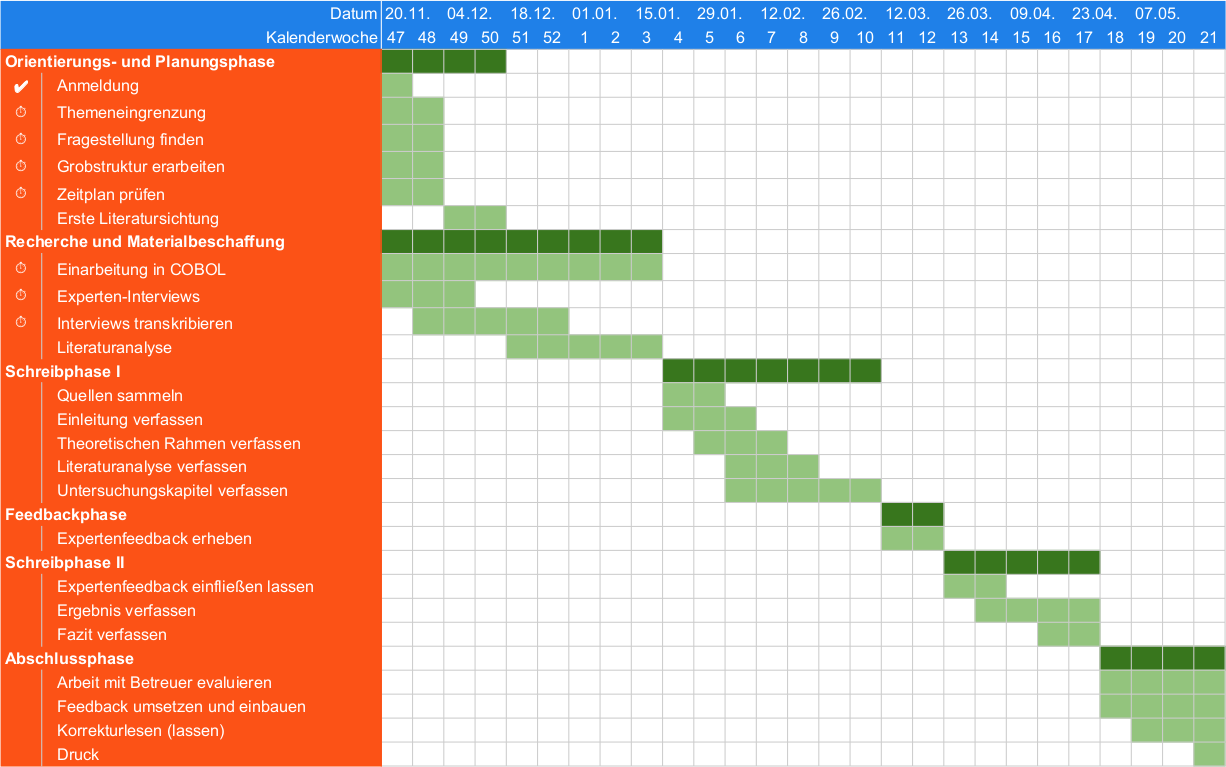
\includegraphics[width=.9\linewidth]{Bilder/Zeitplan}
\end{landscape}
\restoregeometry
	
\end{document}
